\documentclass[12pt]{article}
\usepackage[margin=0.8in]{geometry}
\usepackage{authblk}
\usepackage{amsmath}
\usepackage{caption}
\usepackage{subcaption}
\usepackage{setspace}
\usepackage{graphicx}
\usepackage{epstopdf}
\graphicspath{{graph/}}
\onehalfspacing

\title{\LARGE \textbf{Contrast problem in PDE} \\ \large \textbf{a computational study with Finite Element Method}}
\date{\today}
\author[1]{Simiao Zuo}
\author[2]{Ivo Babuska}
\affil[1]{Department of Computer Science, The University of Texas at Austin}
\affil[2]{Institute for Computational Engineering and Sciences, The University of Texas at Austin}

\begin{document}

\maketitle

\section{Introduction}
The Finite Element Method (FEM) is today without doubt one of the major numerical tools in computational science. This position of pre-eminence has arisen as a result of a number of complementary factors. These include: the requirement for engineers, scientists, financiers and clinicians to be able to simulate and solve numerically ever more complex problems; the results on the theory of finite elements that have been produced by mathematicians since the 1960s, particularly regarding error estimation; and last but by no means least, the inexorable increase in computer power over the last half century and the corresponding increase in the expectations of users.

Many problems in engineering are PDEs with large contrast. These could lead to the system of linear equations with a large scaled condition number. The report analyzes the condition number in connection with different boundary conditions of such problems.

\section{One-dimensional interface problem}
\subsection{The interface problem}
Consider the following interface problem: $$-\frac{d}{dx}(a(x)\frac{du(x)}{dx})=f(x), 0\leq x \leq 1$$
\[
\begin{cases}
u(0)=0 \quad or \quad u'(0)=0 \\
u(1)=0 \quad or \quad u'(1)=0
\end{cases}
\]
where
\[
a(x)=
\begin{cases}
1 & 0 \leq x < \beta \\
A & \beta \leq x \leq 1
\end{cases}
\]

In the interface problem, $x=\beta$ is the position of the interface, and $A$ is the contrast. Homogeneous Dirichlet or Neumann boundary is imposed at each end, i.e. $x=0$ and $x=1$.

For simplification, we take $f(x)=1$ for all the problems.

\subsection{Construction of the exact solution}
\subsubsection{Dirichlet-Dirichlet boundary problem}
By solving the equations
\[
\begin{cases}
-u''(x)=1 & 0 \leq x < \beta \\
-Au''(x)=1 & \beta \leq x \leq 1 \\
\end{cases}
\]
we have a general solution
\begin{equation} \label{eq1}
\begin{cases}
u_{1}(x)=-\frac{x^2}{2}+c_{1}x+c_{2} & 0 \leq x < \beta \\
u_{2}(x)=-\frac{x^2}{2A}+c_{3}x+c_{4} & \beta \leq x \leq 1
\end{cases}
\end{equation}

Homogeneous Dirichlet boundary conditions are imposed at both endpoints, and we impose $u(x)$ to be continuously differentiable at $x=\beta$, thus
\[
\begin{cases}
u_{1}(0)=0, & u_{2}(1)=0 \\
u_{1}(\beta)=u_{2}(\beta), & u_{1}'(\beta)=Au_{2}'(\beta)
\end{cases}
\]

By solving the equations, we have
\[
u(x)=
\begin{cases}
-\frac{x^2}{2}+\frac{\beta^2(A-1)+1}{2(\beta(A-1)+1)}x & 0 \leq x < \beta \\
-\frac{x^2}{2A}+\frac{\beta^2(A-1)+1}{2A(\beta(A-1)+1)}x+\frac{(\beta-\beta^2)(A-1)}{2A(\beta(A-1)+1)} & \beta \leq x \leq 1
\end{cases}
\]

Obviously when the contrast $A$ goes to infinity
\[
u_{A \to \infty}(x)=
\begin{cases}
-\frac{x^2}{2}+\frac{\beta}{2}x & 0 \leq x < \beta \\
0 & \beta \leq x \leq 1
\end{cases}
\]

\subsubsection{Dirichlet-Neumann boundary problem}
In the same way, we have equation $\ref{eq1}$, then we impose homogeneous Dirichlet boundary condition at $x=0$ and homogeneous Neumann boundary condition at $x=1$.

By solving
\[
\begin{cases}
u_{1}(0)=0, & u_{2}'(1)=0 \\
u_{1}(\beta)=u_{2}(\beta), & u_{1}'(\beta)=Au_{2}'(\beta)
\end{cases}
\]
we have
\[
u(x)=
\begin{cases}
-\frac{x^2}{2}+x & 0 \leq x < \beta \\
-\frac{x^2}{2A}+\frac{1}{A}x+\frac{(2\beta-\beta^2)(A-1)}{2A} & \beta \leq x \leq 1
\end{cases}
\]

Obviously when the contrast $A$ goes to infinity
\[
u_{A \to \infty}(x)=
\begin{cases}
-\frac{x^2}{2}+x & 0 \leq x < \beta \\
\frac{2\beta-\beta^2}{2} & \beta \leq x \leq 1
\end{cases}
\]

\subsubsection{Neumann-Dirichlet boundary problem}
Similarly to above, we impose homogeneous Neumann boundary at $x=0$ and homogeneous Dirichlet boundary at $x=1$ on equation $\ref{eq1}$.

By solving
\[
\begin{cases}
u_{1}'(0)=0, & u_{2}(1)=0 \\
u_{1}(\beta)=u_{2}(\beta), & u_{1}'(\beta)=Au_{2}'(\beta)
\end{cases}
\]
we have
\[
u(x)=
\begin{cases}
-\frac{x^2}{2}+\frac{\beta^2(A-1)+1}{2A} & 0 \leq x < \beta \\
-\frac{x^2}{2A}+\frac{1}{2A} & \beta \leq x \leq 1
\end{cases}
\]

When the contrast $A$ goes to infinity, we obtain
\[
u_{A \to \infty}(x)=
\begin{cases}
-\frac{x^2}{2}+\frac{\beta^2}{2} & 0 \leq x < \beta \\
0 & \beta \leq x \leq 1
\end{cases}
\]

\subsection{Construction of the FEM solution}
\subsubsection{Construction of the system of equations}
Consider a uniform mesh on $\Omega=[0,1]$: \\
\setlength{\unitlength}{1cm}
\thicklines
\begin{picture}(0,2.8)(-5,0)
\put(0,0){\line(1,0){8}}
\put(0,0){\line(0,1){2}}
\put(2,0){\line(0,1){2}}
\put(8,0){\line(0,1){2}}
\put(0,2){\line(1,-1){2}}
\put(2,2){\line(-1,-1){2}}
\put(2,2){\line(1,-1){2}}
\put(8,2){\line(-1,-1){2}}
\put(4.6,1){......}
\put(0.8,-0.4){$\tau_{1}$}
\put(2.8,-0.4){$\tau_{2}$}
\put(6.8,-0.4){$\tau_{n}$}
\put(-0.2,2.1){$\Phi_{1}$}
\put(1.8,2.1){$\Phi_{2}$}
\put(7.6,2.1){$\Phi_{n+1}$}
\end{picture} \\ \\
where
\[
\Phi_{i}(x)=
\begin{cases}
\frac{x-x_{i-1}}{h} & x_{i-1} \leq x <x_{i} \\
\frac{x_{i+1}-x}{h} & x_{i} \leq x<x_{i+1} \\
0 & otherwise
\end{cases}
\] \\
are the shape functions, and the FEM solution $u(x)=\sum_{i}u_{i}\Phi_{i}(x)$.

Denote $h$ the size of each element. Since we are taking a uniform mesh, $h$ is a constant, then $N=\frac{1}{h}$ is the number of elements. Denote function $B(u,v)=\int_{0}^{1}a(x)u'(x)v'(x)dx$.

We can construct the system of equations
\[
\begin{bmatrix}
B(\Phi_{1}, \Phi_{1}) & B(\Phi_{1}, \Phi_{2}) & \hdots & B(\Phi_{1}, \Phi_{n+1}) \\
B(\Phi_{2}, \Phi_{1}) & B(\Phi_{2}, \Phi_{2}) & \hdots & B(\Phi_{2}, \Phi_{n+1}) \\
\vdots & \vdots & \ddots & \vdots \\
B(\Phi_{n+1}, \Phi_{1}) & B(\Phi_{n+1}, \Phi_{2}) & \hdots & B(\Phi_{n+1}, \Phi_{n+1})
\end{bmatrix}
\begin{bmatrix}
u_{1} \\
u_{2} \\
\vdots \\
u_{n+1}
\end{bmatrix}
=
\begin{bmatrix}
\int_{0}^{1}f\Phi_{1}dx \\
\int_{0}^{1}f\Phi_{2}dx \\
\vdots \\
\int_{0}^{1}f\Phi_{n+1}dx
\end{bmatrix}
\]

Construct the global stiffness matrix element by element. For the elements that don't contain the interface, notice that each element $\tau_{i}$ is only connected to $\Phi_{i}$ and $\Phi_{i+1}$, thus we have
$$B(\Phi_{i},\Phi_{j})=0 \quad |i-j|>1$$
$$B(\Phi_{i},\Phi_{i})=B(\Phi_{i+1},\Phi_{i+1})=\int_{\tau}\frac{a}{h^2}dx=\frac{a}{h}$$
$$B(\Phi_{i},\Phi_{i+1})=B(\Phi_{i+1},\Phi_{i})=\int_{\tau}-\frac{a}{h^2}dx=-\frac{a}{h}$$
Therefore, for each element that don't contain the interface, the local stiffness matrix is
\[
\textbf{K}=
\begin{bmatrix}
\frac{a}{h} & -\frac{a}{h} \\
-\frac{a}{h} & \frac{a}{h}
\end{bmatrix}
\]
Now consider the element that contains the interface \\
\setlength{\unitlength}{1cm}
\thicklines
\begin{picture}(0,2.5)(-8,0)
\put(0,1){\line(1,0){2}}
\put(1,0){\line(0,1){2}}
\put(0.01,1){\line(0,1){0.1}}
\put(1.99,1){\line(0,1){0.1}}
\put(-0.2,0.7){$x_{i}$}
\put(1.7,0.7){$x_{i+1}$}
\put(1.1,0){$\beta$}
\put(0.4,1.1){\small$1$}
\put(1.4,1.1){\small$A$}
\end{picture} \\
Here obviously $x_{i}=\lfloor \beta \rfloor$ and $i=\lceil{N\beta}\rceil$. Then
$$B(\Phi_{i},\Phi_{i})=B(\Phi_{i+1},\Phi_{i+1})=\int_{x_{i}}^{\beta}\frac{1}{h^2}dx+\int_{\beta}^{x_{i+1}}\frac{A}{h^2}dx=\frac{\beta-x_{i}+A(x_{i+1}-\beta)}{h^2}$$
$$B(\Phi_{i},\Phi_{i+1})=B(\Phi_{i+1},\Phi_{i})=\int_{x_{i}}^{\beta}-\frac{1}{h^2}dx+\int_{\beta}^{x_{i+1}}-\frac{A}{h^2}dx=-\frac{\beta-x_{i}+A(x_{i+1}-\beta)}{h^2}$$
Therefore, for the element that contains the interface, the local stiffness matrix is
\[
\doublespacing
\textbf{K}=
\begin{bmatrix}
\frac{\beta-x_{i}+A(x_{i+1}-\beta)}{h^2} & -\frac{\beta-x_{i}+A(x_{i+1}-\beta)}{h^2} \\
-\frac{\beta-x_{i}+A(x_{i+1}-\beta)}{h^2} & \frac{\beta-x_{i}+A(x_{i+1}-\beta)}{h^2}
\end{bmatrix}
\]

Now construct the load vector of each element
\[
\textbf{f}=
\begin{bmatrix}
\int_{\tau}\frac{x-x_{i-1}}{h}dx \\
\int_{\tau}\frac{x_{i+1}-x}{h}dx
\end{bmatrix}
=
\begin{bmatrix}
\frac{h}{2} \\
\frac{h}{2}
\end{bmatrix}
\]

Then we can construct the unconstrained system of equations (with Neumann-Neumann boundary conditions)
\[
\doublespacing
\begin{bmatrix}
\frac{1}{h} & -\frac{1}{h} \\
-\frac{1}{h} & \frac{2}{h} & -\frac{1}{h} \\
& \ddots & \ddots & \ddots\\
&& -\frac{1}{h} & \frac{2}{h} & -\frac{1}{h}\\
&&& -\frac{1}{h} & (\frac{1}{h}+\frac{\beta-x_{i}+A(x_{i+1}-\beta)}{h^2}) & -\frac{\beta-x_{i}+A(x_{i+1}-\beta)}{h^2}\\
&&&& -\frac{\beta-x_{i}+A(x_{i+1}-\beta)}{h^2} & (\frac{A}{h}+\frac{\beta-x_{i}+A(x_{i+1}-\beta)}{h^2}) & -\frac{A}{h}\\
&&&&& -\frac{A}{h} & \frac{2A}{h} & -\frac{A}{h}\\
&&&&&& \ddots & \ddots & \ddots\\
&&&&&&& -\frac{A}{h} & \frac{2A}{h} & -\frac{A}{h}\\
&&&&&&&&  -\frac{A}{h} & \frac{A}{h}
\end{bmatrix}
\begin{bmatrix}
u_{1}\\
u_{2}\\
\vdots\\
\vdots\\
\vdots\\
\vdots\\
\vdots\\
\vdots\\
u_{n}\\
u_{n+1}
\end{bmatrix}=
\begin{bmatrix}
\frac{h}{2}\\
h\\
\vdots\\
\vdots\\
\vdots\\
\vdots\\
\vdots\\
\vdots\\
h\\
\frac{h}{2}
\end{bmatrix}
\]

\subsubsection{FEM solution of Dirichlet-Dirichlet problem}
When imposing homogeneous Dirichlet boundaries at both endpoints, the system of equations become
\[
\begin{bmatrix}
\frac{2}{h} & -\frac{1}{h} \\
-\frac{1}{h} & \frac{2}{h} & -\frac{1}{h} \\
& \ddots & \ddots & \ddots \\
&& -\frac{A}{h} & \frac{2A}{h} & -\frac{A}{h} \\
&&& -\frac{A}{h} & \frac{2A}{h}
\end{bmatrix}
\begin{bmatrix}
u_{2} \\
u_{3} \\
\vdots \\
u_{n-1} \\
u_{n}
\end{bmatrix}
=
\begin{bmatrix}
h \\
h \\
\vdots \\
h \\
h
\end{bmatrix}
\]
with $u_{1}=0$ and $u_{n+1}=0$.

By solving the system of equations, we obtain the FEM solution.
\begin{figure}[h!]
\centering
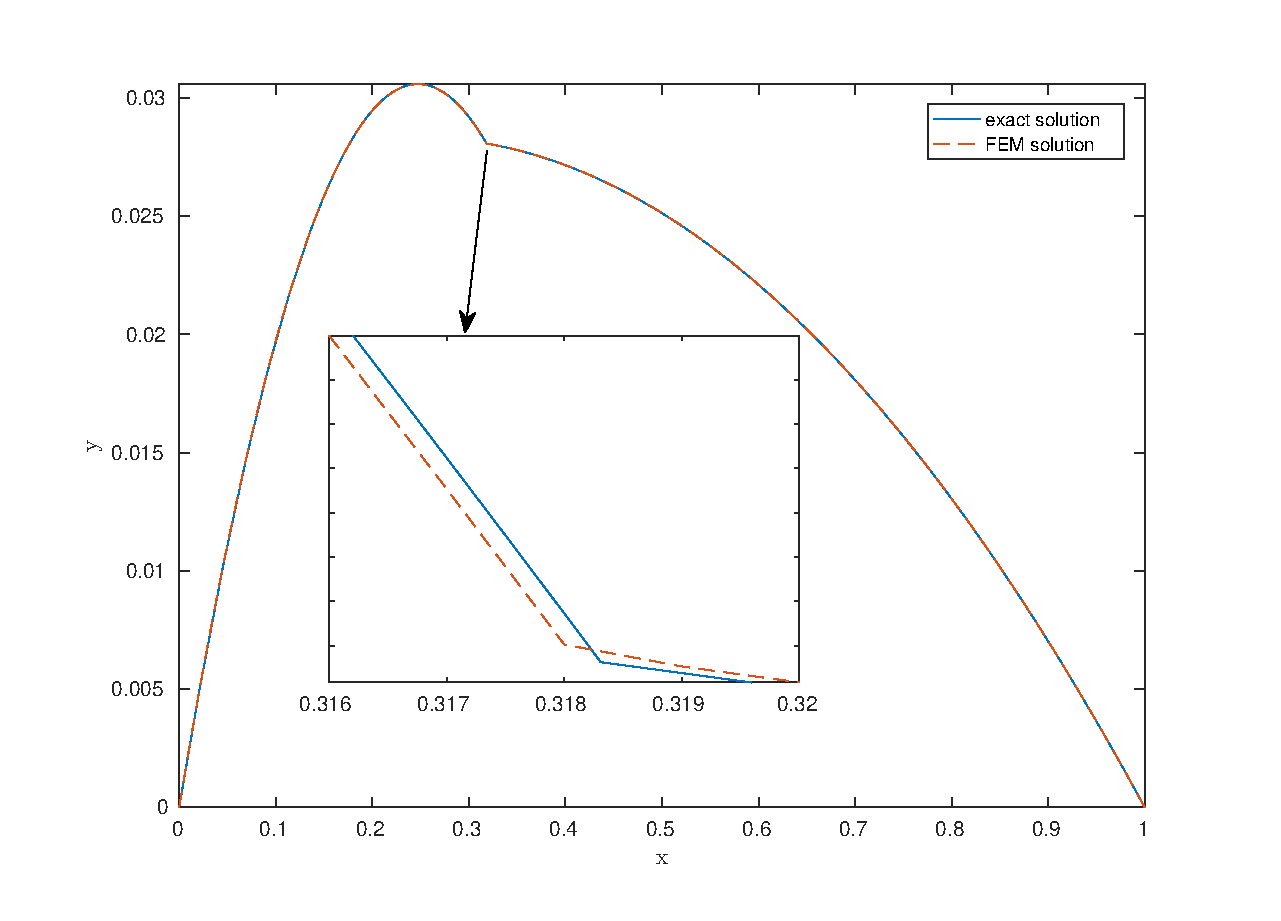
\includegraphics[scale=0.6]{FEM-pi-DD}
\caption{FEM solution, $h=10^{-3},\beta=\frac{1}{\pi},A=10$, Dirichlet-Dirichlet boundary}
\end{figure}
\pagebreak
\begin{figure}[h!]
\centering
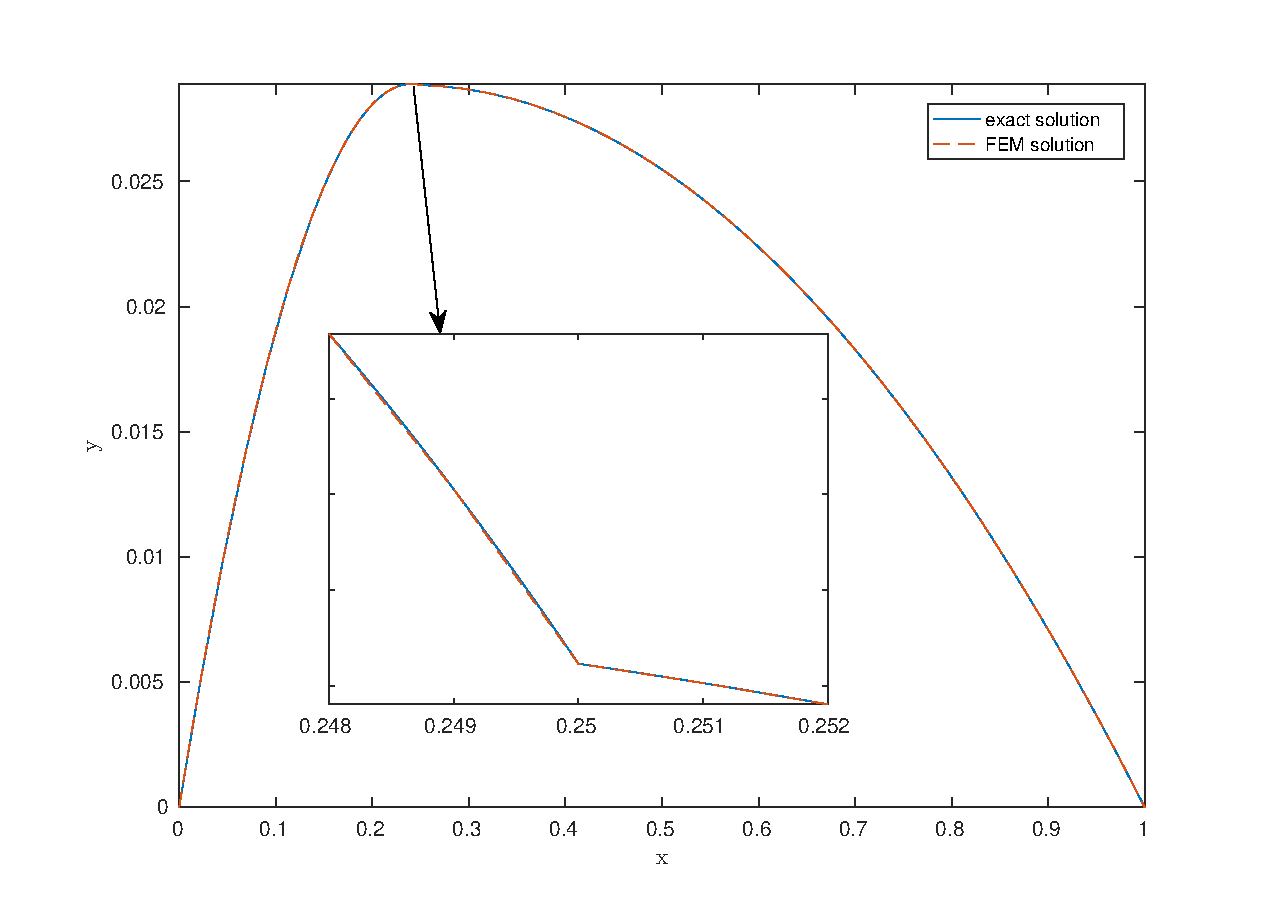
\includegraphics[scale=0.6]{FEM-4-DD}
\caption{FEM solution, $h=10^{-3},\beta=\frac{1}{4},A=10$, Dirichlet-Dirichlet boundary}
\end{figure}

We can see the different behavior of the FEM solution when the position of the interface changes, i.e. from $\frac{1}{\pi}$ to $\frac{1}{4}$. This is due to the fact that when taking $\beta=\frac{1}{\pi}$, the interface is always between two nodal points, but when taking $\beta=\frac{1}{4}$, the interface can be on a nodal point. The same happens when imposing other types of boundary conditions.

\subsubsection{FEM solution of Dirichlet-Neumann problem}
Similarly, the system of equations are
\[
\begin{bmatrix}
\frac{2}{h} & -\frac{1}{h} \\
-\frac{1}{h} & \frac{2}{h} & -\frac{1}{h} \\
& \ddots & \ddots & \ddots \\
&& -\frac{A}{h} & \frac{2A}{h} & -\frac{A}{h} \\
&&& -\frac{A}{h} & \frac{A}{h}
\end{bmatrix}
\begin{bmatrix}
u_{2} \\
u_{3} \\
\vdots \\
u_{n} \\
u_{n+1}
\end{bmatrix}
=
\begin{bmatrix}
h \\
h \\
\vdots \\
h \\
\frac{h}{2}
\end{bmatrix}
\]
with $u_{1}=0$. We can then construct the FEM solution

\begin{figure}[h!]
\centering
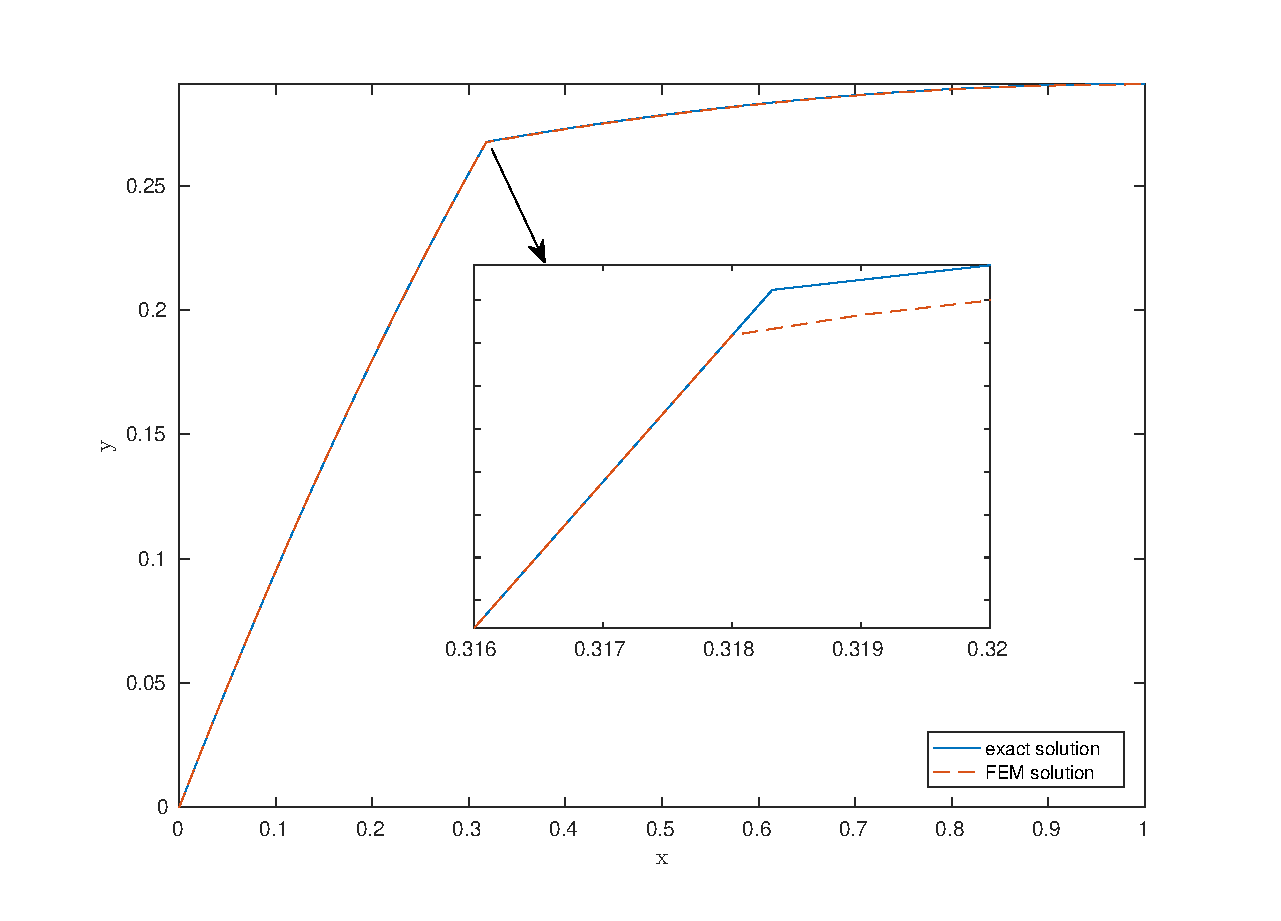
\includegraphics[scale=0.6]{FEM-pi-DN}
\caption{FEM solution, $h=10^{-3},\beta=\frac{1}{\pi},A=10$, Dirichlet-Neumann boundary}
\end{figure}
\pagebreak
\begin{figure}[h!]
\centering
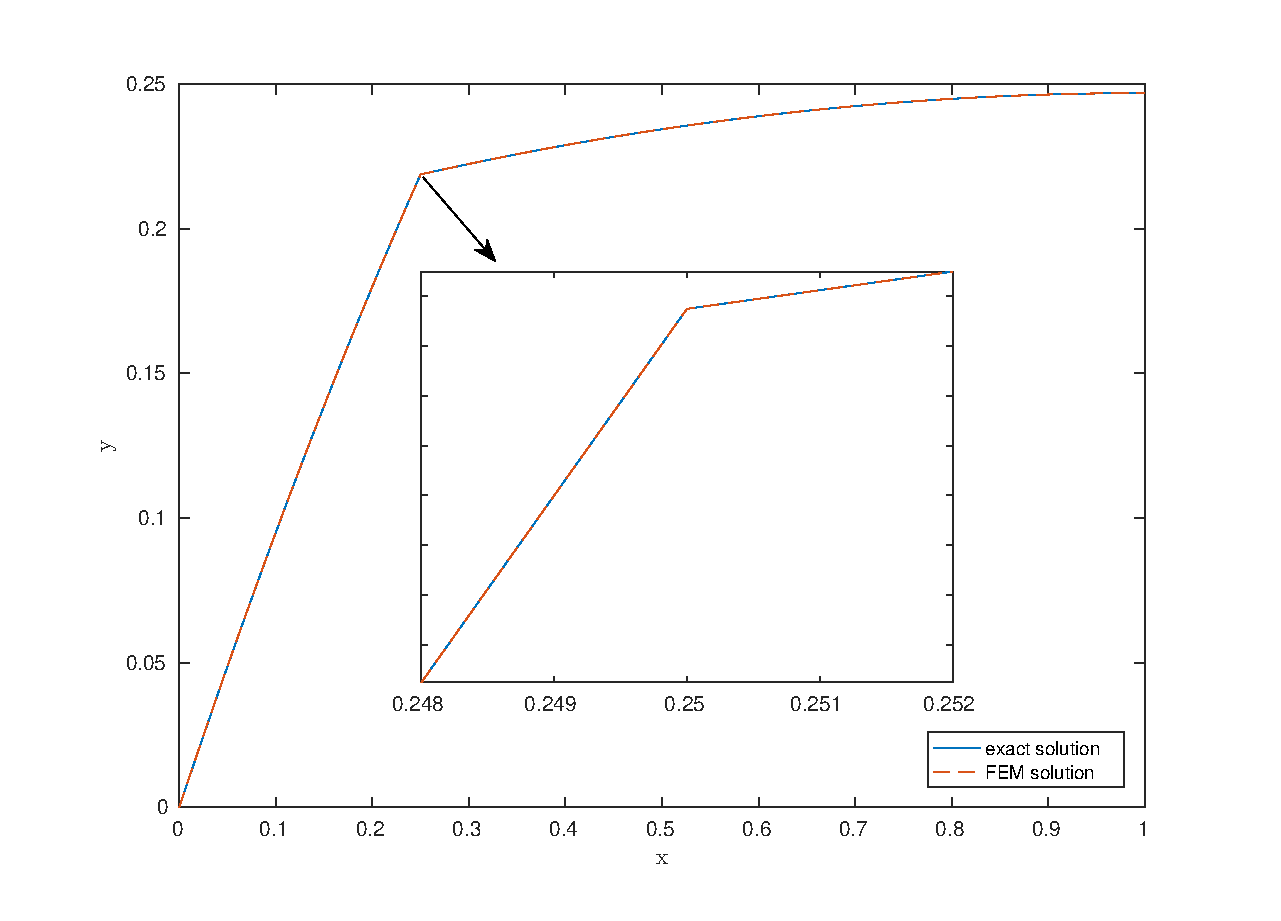
\includegraphics[scale=0.6]{FEM-4-DN}
\caption{FEM solution, $h=10^{-3},\beta=\frac{1}{4},A=10$, Dirichlet-Neumann boundary}
\end{figure}

\subsubsection{FEM solution of Neumann-Dirichlet problem}
Now the system of equations are
\[
\begin{bmatrix}
\frac{1}{h} & -\frac{1}{h} \\
-\frac{1}{h} & \frac{2}{h} & -\frac{1}{h} \\
& \ddots & \ddots & \ddots \\
&& -\frac{A}{h} & \frac{2A}{h} & -\frac{A}{h} \\
&&& -\frac{A}{h} & \frac{2A}{h}
\end{bmatrix}
\begin{bmatrix}
u_{1} \\
u_{2} \\
\vdots \\
u_{n-1} \\
u_{n}
\end{bmatrix}
=
\begin{bmatrix}
\frac{h}{2} \\
h \\
\vdots \\
h \\
h
\end{bmatrix}
\]
with $u_{n+1}=0$.

The FEM solution is
\begin{figure}[h!]
\centering
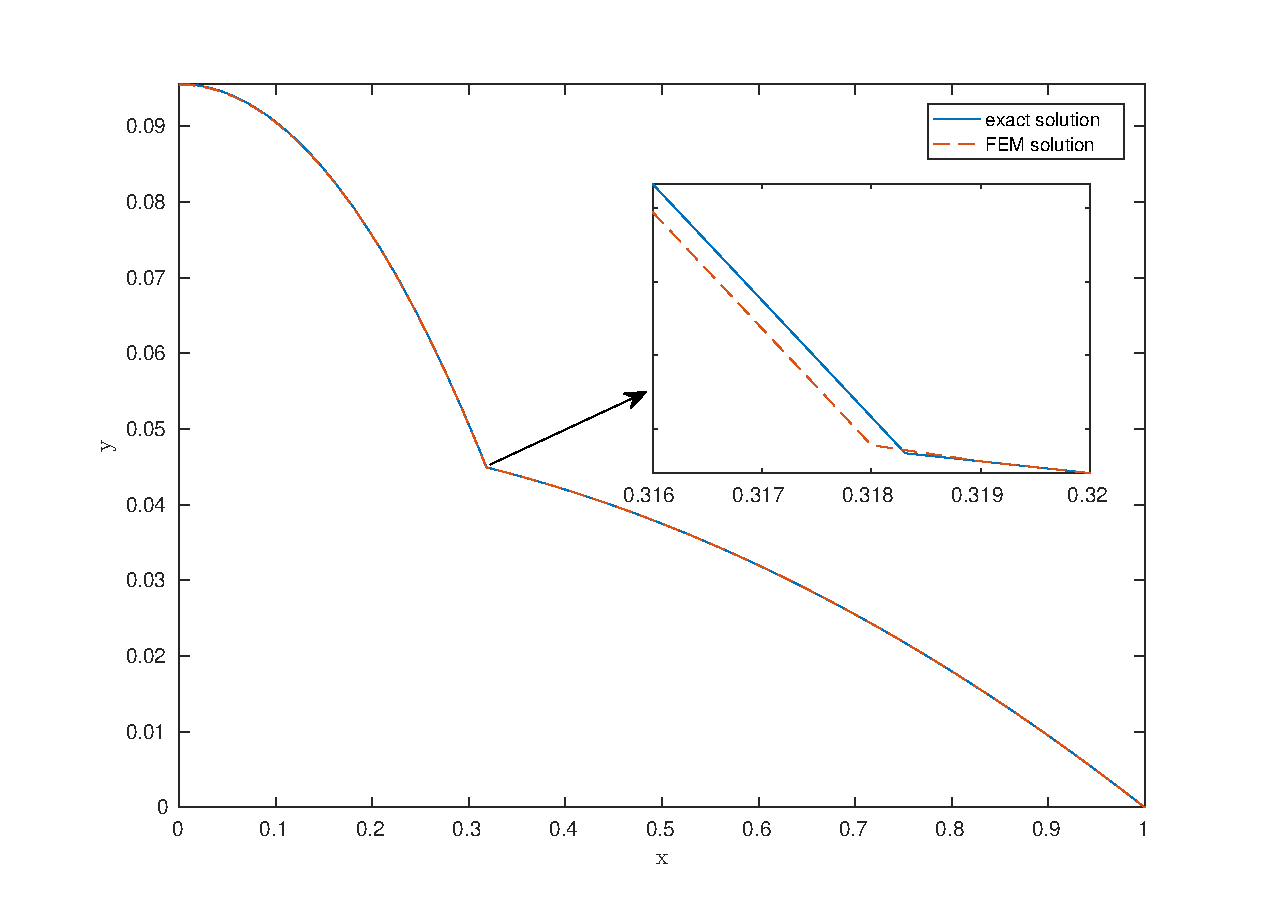
\includegraphics[scale=0.6]{FEM-pi-ND}
\caption{FEM solution, $h=10^{-3},\beta=\frac{1}{\pi},A=10$, Neumann-Dirichlet boundary}
\end{figure}
\pagebreak
\begin{figure}[h!]
\centering
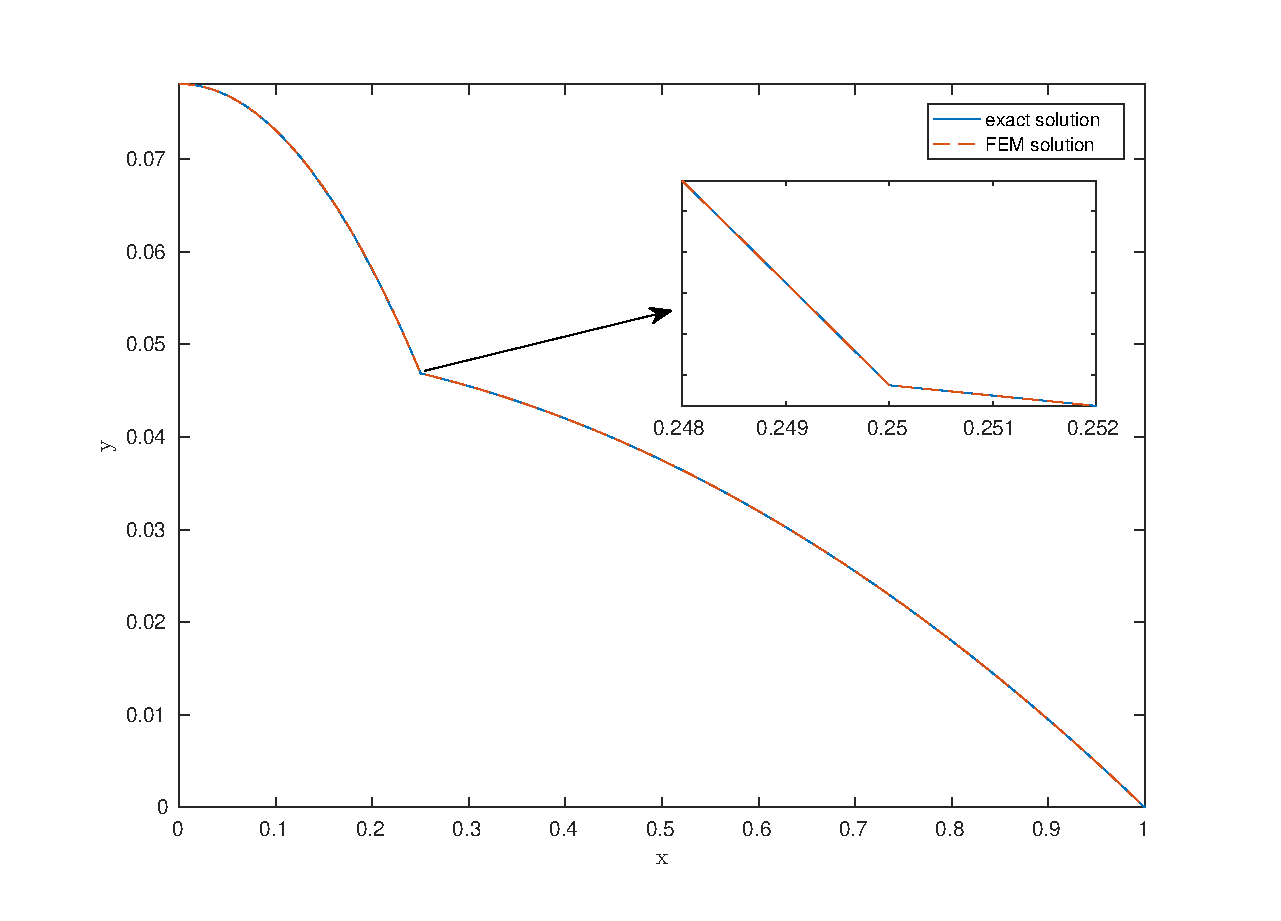
\includegraphics[scale=0.6]{FEM-4-ND}
\caption{FEM solution, $h=10^{-3},\beta=\frac{1}{4},A=10$, Neumann-Dirichlet boundary}
\end{figure}

\subsection{Error analysis of FEM solution}
\subsubsection{Error of Dirichlet-Dirichlet problem}
The error is computed piecewise in energy norm
$$e^2=B(u-u_{h},u-u_{h})=\sum_{i}\int_{x_{i}}^{x_{i+1}}a(x)((u-u_{h})')^2dx$$
where $u$ is the exact solution, and $u_{h}$ is the FEM solution.
\begin{figure}[h!]
\centering
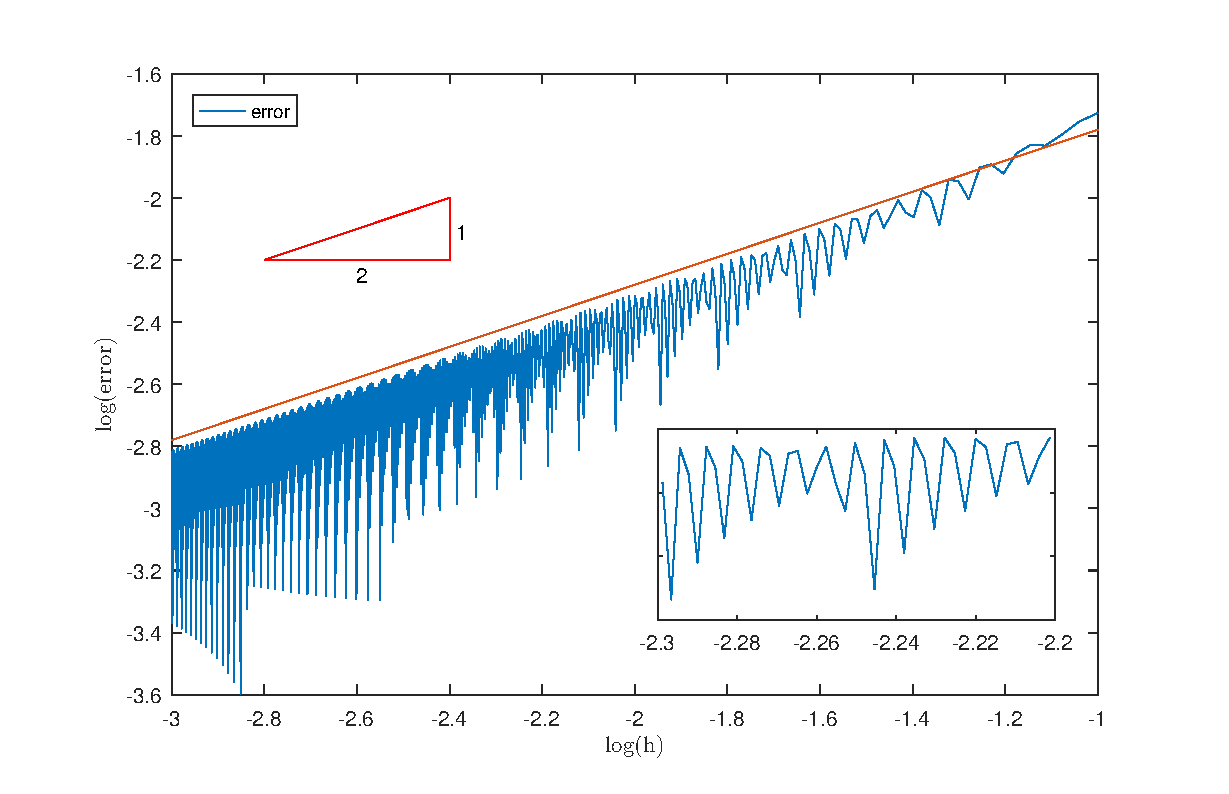
\includegraphics[scale=0.7]{error-pi-DD}
\caption{Error of FEM solution, $\beta=\frac{1}{\pi},A=10$, Dirichlet-Dirichlet boundary}
\label{fig-e-pi-DD}
\end{figure}

\begin{figure}[h!]
\centering
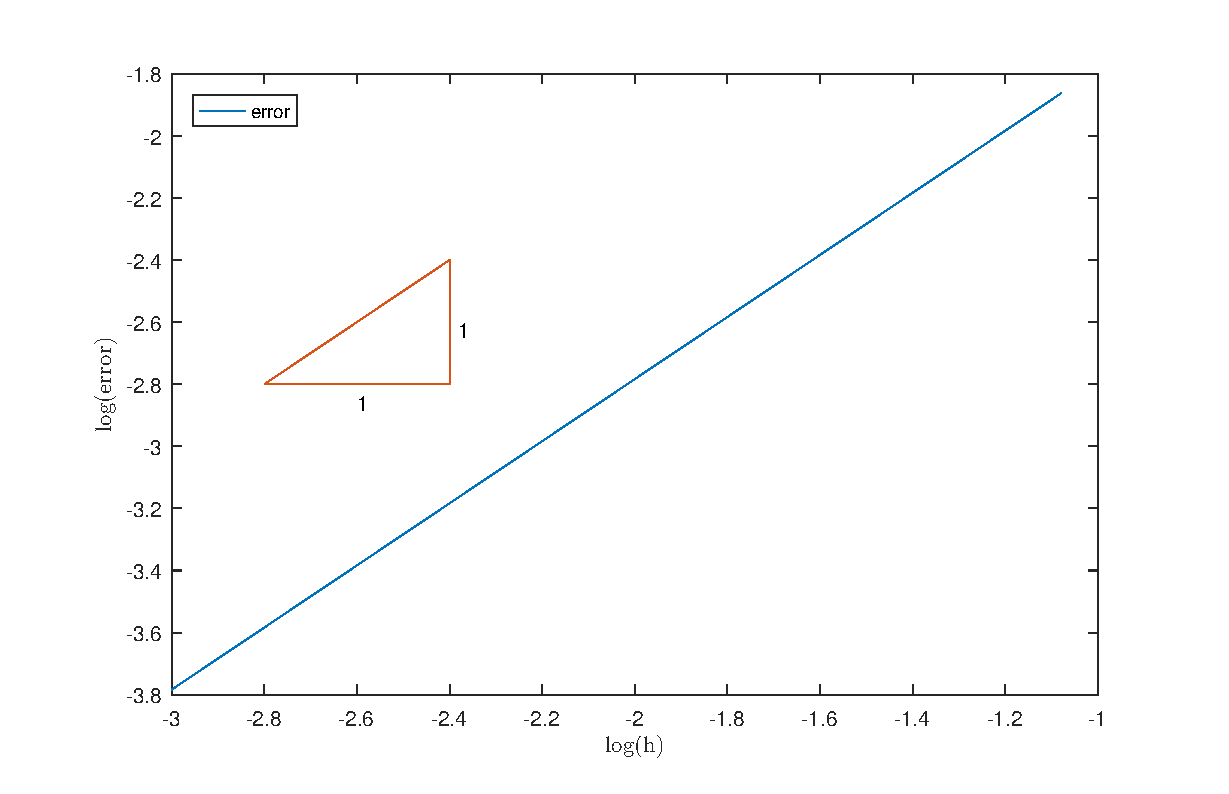
\includegraphics[scale=0.7]{error-4-DD}
\caption{Error of FEM solution, $h=\frac{1}{4k},\beta=\frac{1}{4},A=10$, Dirichlet-Dirichlet boundary}
\label{fig-e-4-DD}
\end{figure}

We can see that the error of FEM solution behaves differently for interface $\beta=\frac{1}{\pi}$ and $\beta=\frac{1}{4}$, which is intuitively shown in the comparison of the FEM solution with the exact solution. The reason is that for the elements that don't contain the interface, $error \propto h$, and for the element that contains the interface, $error \propto \sqrt{h}$. Notice that in figure $\ref{fig-e-4-DD}$, the number of elements $N$ is always a multiplication of $4$ and we take the interface $\beta=\frac{1}{4}$. Thus the interface is always on a nodal point, therefore $e \propto h$. On the other hand, when taking the interface $\beta=\frac{1}{\pi}$, it's always contained in one of the elements, the combined consequence is that $e \propto \sqrt{h}$.

As the graphs illustrated, when taking $\beta=\frac{1}{4}$, the error of FEM solution converges linearly to $0$ at the rate of $h$. And when taking $\beta=\frac{1}{\pi}$, the error converges to $0$ at the rate of $\sqrt{h}$. Worth noticing that when taking $\beta=\frac{1}{\pi}$, the error does not converges linearly, and even not converging locally, as shown by the small graph in figure $\ref{fig-e-pi-DD}$. This is also true for other types of boundary conditions.

Now consider a large contrast.
\pagebreak
\begin{figure}[h!]
\centering
\begin{subfigure}{0.4\textwidth}
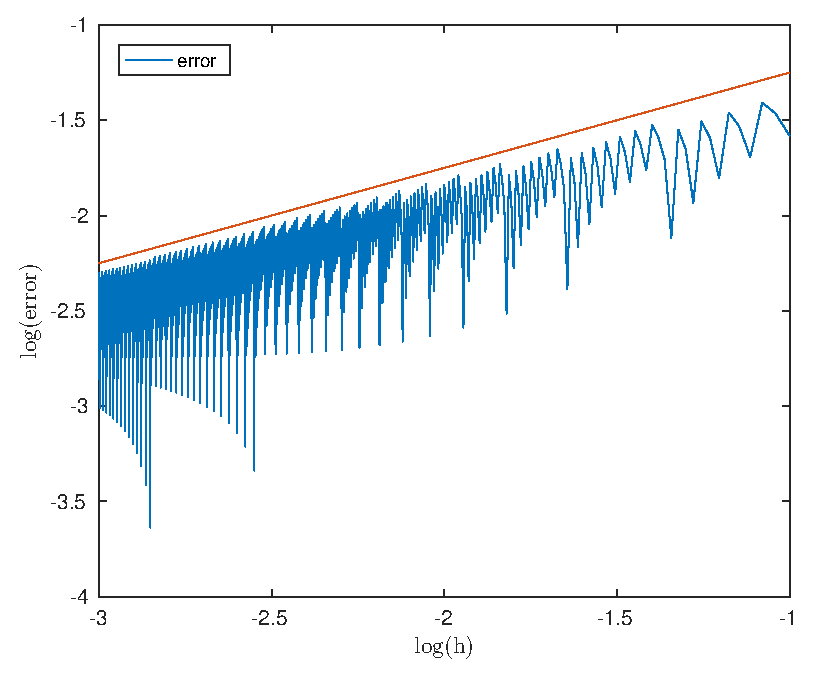
\includegraphics[width=\textwidth]{error-pi-DD-12}
\caption{$\beta=\frac{1}{\pi}$}
\end{subfigure}
\hfill
\begin{subfigure}{0.4\textwidth}
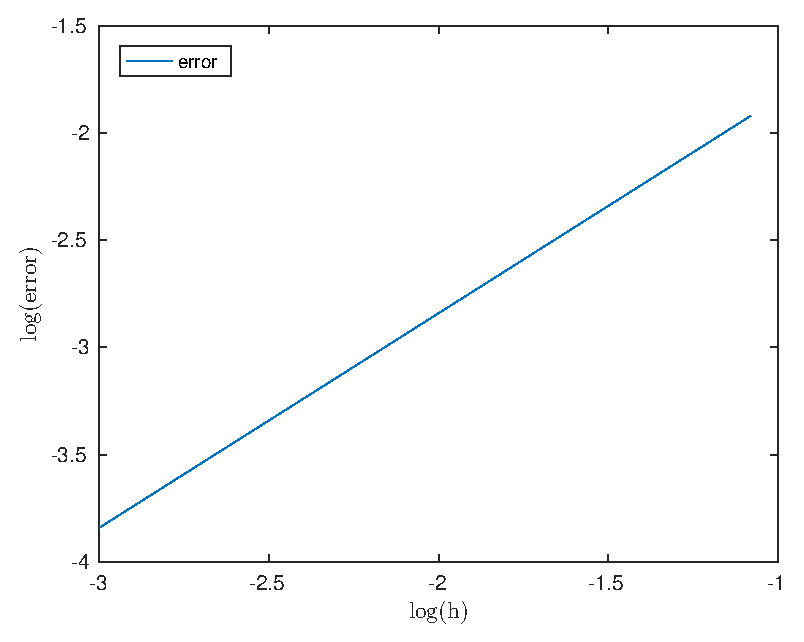
\includegraphics[width=\textwidth]{error-4-DD-12}
\caption{$h=\frac{1}{4k},\beta=\frac{1}{4}$}
\end{subfigure}
\caption{Error of FEM solution,$A=10^{12}$, Dirichlet-Dirichlet boundary}
\end{figure} \\
Notice that increasing the contrast does not have a significant influence on the behavior of error.

\subsubsection{Error of Dirichlet-Neumann problem}
In the same way we compute the error of FEM solution in energy norm.
\begin{figure}[h!]
\centering
\begin{subfigure}{0.4\textwidth}
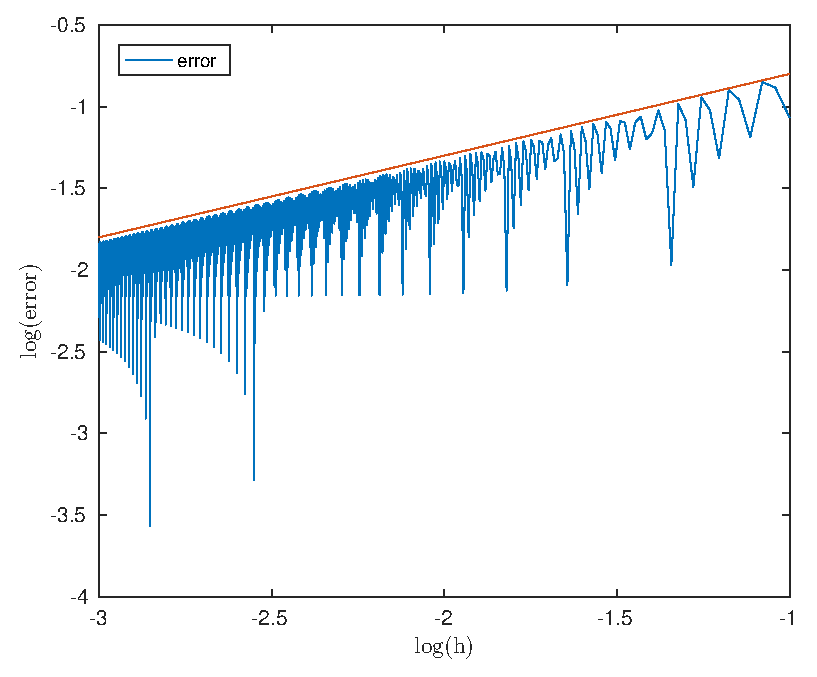
\includegraphics[width=\textwidth]{error-pi-DN}
\caption{$\beta=\frac{1}{\pi}$}
\end{subfigure}
\hfill
\begin{subfigure}{0.4\textwidth}
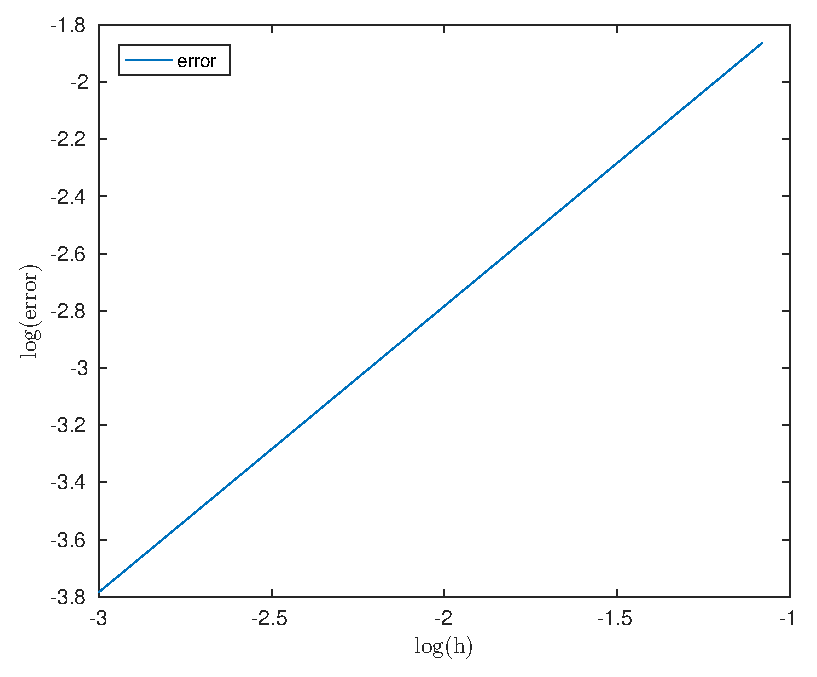
\includegraphics[width=\textwidth]{error-4-DN}
\caption{$h=\frac{1}{4k},\beta=\frac{1}{4}$}
\end{subfigure}
\caption{Error of FEM solution,$A=10$, Dirichlet-Neumann boundary}
\end{figure}

In comparison, error is also computed with a large contrast.
\begin{figure}[h!]
\centering
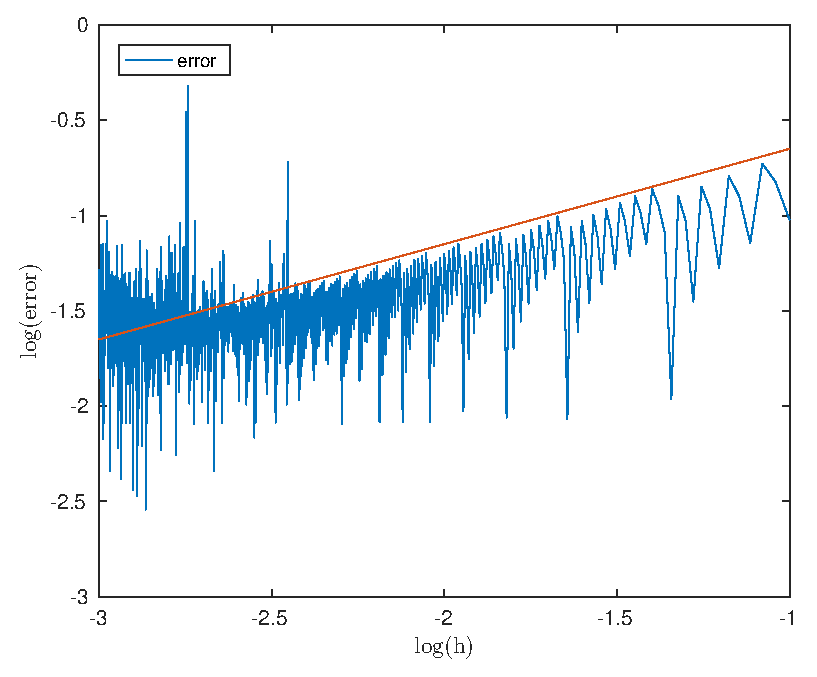
\includegraphics[scale=0.7]{error-pi-DN-12}
\caption{Error of FEM solution,$\beta=\frac{1}{\pi},A=10^{12}$, Dirichlet-Neumann boundary}
\label{fig-e-pi-DN}
\end{figure}
\pagebreak

\begin{figure}[h!]
\centering
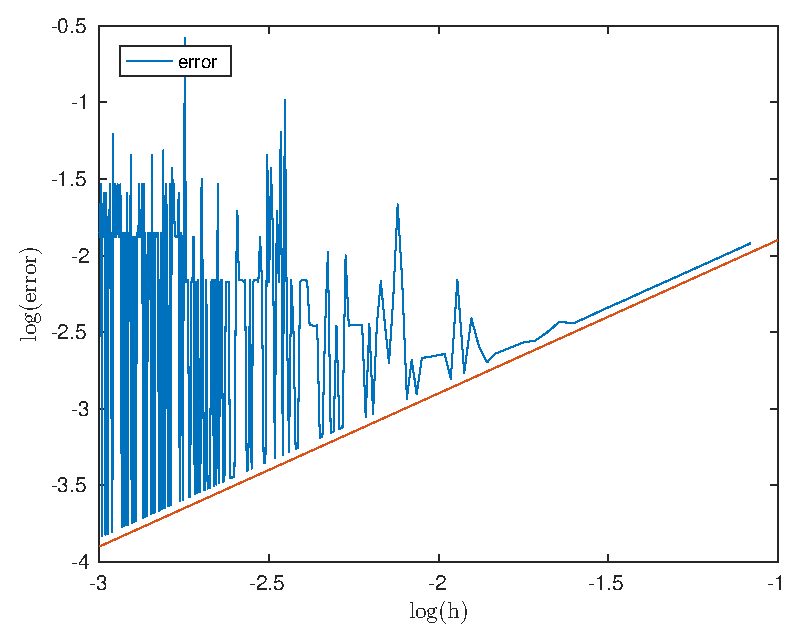
\includegraphics[scale=0.7]{error-4-DN-12}
\caption{Error of FEM solution,$h=\frac{1}{4k},\beta=\frac{1}{4},A=10^{12}$, Dirichlet-Neumann boundary}
\label{fig-e-4-DN}
\end{figure}

For a small contrast, i.e. $A=10$, the error behaves similarly to the one of Dirichlet-Dirichlet problem. When taking $\beta=\frac{1}{\pi}$, the error converges to $0$ at the rate of $\sqrt{h}$. And when taking $\beta=\frac{1}{4}$, the error converges to $0$ at the rate of $h$. However, for a large contrast, i.e. $A=10^{12}$, the error is unpredictable for $h$ smaller than a certain number, as illustrated in figure $\ref{fig-e-pi-DN}$ and $\ref{fig-e-4-DN}$.

This is the effect of the round-off error in computations. Note that this error is of order $10^{-2}$ when $h=\frac{1}{300}$ although the computation is in double precision.

\subsubsection{Error of Neumann-Dirichlet problem}
Similarly, the error of FEM solution, both with small contrast and with large contrast, is computed in energy norm.

\begin{figure}[h!]
\centering
\begin{subfigure}{0.4\textwidth}
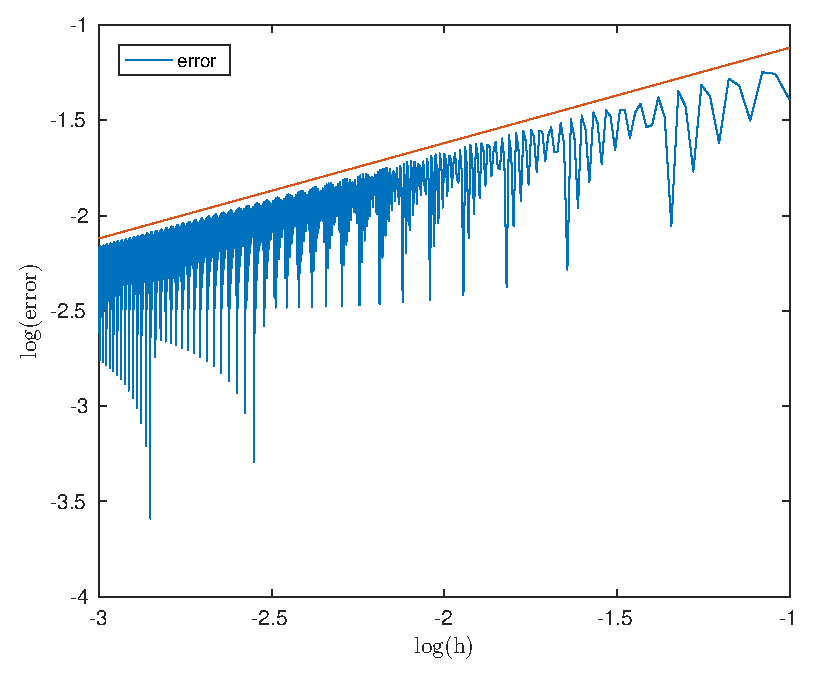
\includegraphics[width=\textwidth]{error-pi-ND}
\caption{$\beta=\frac{1}{\pi}$}
\end{subfigure}
\hfill
\begin{subfigure}{0.4\textwidth}
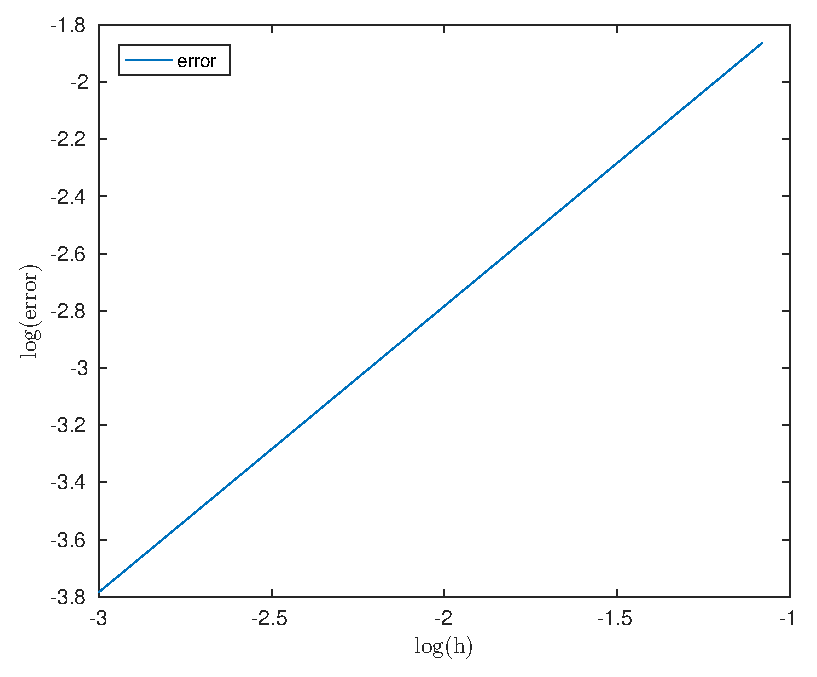
\includegraphics[width=\textwidth]{error-4-ND}
\caption{$h=\frac{1}{4k},\beta=\frac{1}{4}$}
\end{subfigure}
\caption{Error of FEM solution,$A=10$, Neumann-Dirichlet boundary}
\end{figure}

\begin{figure}[h!]
\centering
\begin{subfigure}{0.4\textwidth}
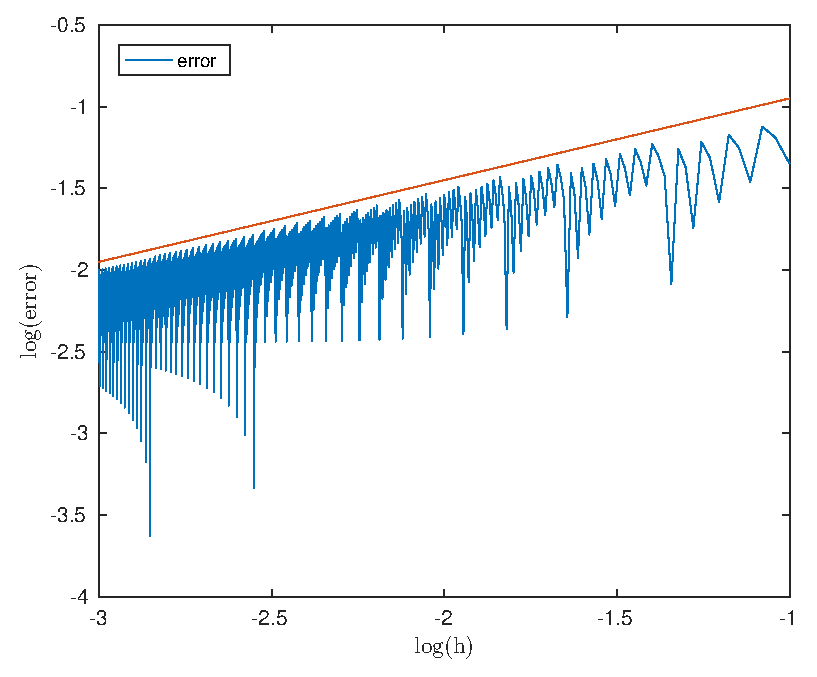
\includegraphics[width=\textwidth]{error-pi-ND-12}
\caption{$\beta=\frac{1}{\pi}$}
\end{subfigure}
\hfill
\begin{subfigure}{0.4\textwidth}
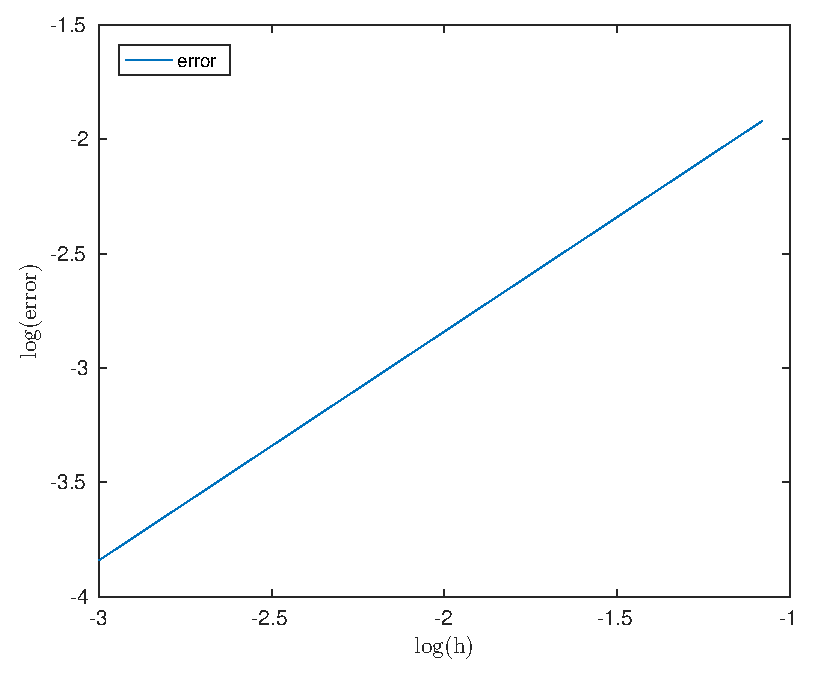
\includegraphics[width=\textwidth]{error-4-ND-12}
\caption{$h=\frac{1}{4k},\beta=\frac{1}{4}$}
\end{subfigure}
\caption{Error of FEM solution,$A=10^{12}$, Neumann-Dirichlet boundary}
\end{figure}

Like in Dirichlet-Dirichlet problem, even with large contrast, the error still converges to $0$ without any disturbance.

\subsection{Scaled condition number of global stiffness matrix}
As shown above, when having a large contrast, i.e. $A=10^{12}$, the error of FEM solution is unpredictable. The reason is that we cannot solve the system of equations accurately, numerical experiments are conducted to show the reason.

First we scaled the global stiffness matrix.
$$\textbf{K}^{*}=\textbf{DKD}$$
where
$$\textbf{D}_{i,i}=\frac{1}{\sqrt{\textbf{K}_{i,i}}} $$
$$\textbf{D}_{i,j}=0 \quad i \neq j$$
so that in this way, all the diagonal elements $\textbf{K}^{*}_{i,i}=1$.

After scaling, the system
$$\textbf{Ku}=\textbf{f}$$
becomes
$$\textbf{D}^{-1}\textbf{K}^{*}\textbf{D}^{-1}\textbf{u}=\textbf{f}$$
and thus
$$\textbf{K}^{*}\textbf{y}=\textbf{Df} \quad \quad \textbf{u}=\textbf{Dy}$$

Notice that by solving the new system, we obtain basically the same result as solving the system $\textbf{Ku}=\textbf{f}$. As a matter of fact, if every $\textbf{D}_{i,j}$ is power of 2, then solving the scaled system and the unscaled system will yield the exact same results. Therefore, scaling the global stiffness matrix doesn't change the FEM solution nor the error, but in this way, we significantly decreases the condition number of the global stiffness matrix.

For simplicity, consider the global stiffness matrix with interface $\beta=\frac{1}{4}$
\[
\doublespacing
\textbf{K}=
\begin{bmatrix}
\frac{1}{h} & -\frac{1}{h} \\
-\frac{1}{h} & \frac{2}{h} & -\frac{1}{h} \\
& \ddots & \ddots & \ddots \\
&& -\frac{1}{h} & \frac{2}{h} & -\frac{1}{h} \\
&&& -\frac{1}{h} & \frac{1+A}{h} & -\frac{A}{h} \\
&&&& -\frac{A}{h} & \frac{2A}{h} & -\frac{A}{h} \\
&&&&& \ddots & \ddots & \ddots \\
&&&&&& -\frac{A}{h} & \frac{2A}{h} & -\frac{A}{h} \\
&&&&&&& -\frac{A}{h} & \frac{A}{h}
\end{bmatrix}
\]
then take such a $\textbf{D}$ to scale the global stiffness matrix
\[
\textbf{D}=
\begin{bmatrix}
\sqrt{h} \\
& \sqrt{\frac{h}{2}} \\
&& \ddots \\
&&& \sqrt{\frac{h}{2}} \\
&&&& \sqrt{\frac{h}{1+A}} \\
&&&&& \sqrt{\frac{h}{2A}} \\
&&&&&& \ddots \\
&&&&&&& \sqrt{\frac{h}{2A}} \\
&&&&&&&& \sqrt{\frac{h}{A}}   
\end{bmatrix}
\]

Consider only the elements that contain the interface and the global stiffness matrix of those elements \\
\setlength{\unitlength}{1cm}
\thicklines
\begin{picture}(0,2.5)(-7,0)
\put(0,1){\line(1,0){4}}
\put(2,0){\line(0,1){2}}
\put(0,1){\line(0,1){0.1}}
\put(4,1){\line(0,1){0,1}}
\put(2.1,0){$\beta$}
\put(0.9,0.7){$\tau_i$}
\put(2.5,0.7){$\tau_{i+1}$}
\end{picture} \\
\[
\textbf{K}_{small}=
\begin{bmatrix}
\frac{2}{h} & -\frac{1}{h} \\
-\frac{1}{h} & \frac{1+A}{h} & -\frac{A}{h} \\
& -\frac{A}{h} & \frac{2A}{h} \\
\end{bmatrix}
\]
this matrix is scaled by multiplying
\[
\textbf{D}_{small}=
\begin{bmatrix}
\sqrt{\frac{h}{2}} \\
& \sqrt{\frac{h}{1+A}} \\
&& \sqrt{\frac{h}{2A}} \\
\end{bmatrix}
\]
then
\[
\textbf{K}_{small}^{*}=\textbf{D}_{small}\textbf{K}_{small}\textbf{D}_{small}=
\begin{bmatrix}
1 & -\frac{1}{\sqrt{2(1+A)}} \\
-\frac{1}{\sqrt{2(1+A)}} & 1 & -\frac{A}{\sqrt{2(1+A)}} \\
& -\frac{A}{\sqrt{2(1+A)}} & 1
\end{bmatrix}
\]
obviously when the contrast $A$ goes to infinity
\[
\lim_{A \to \infty}\textbf{K}_{small}^{*}=
\begin{bmatrix}
1 & 0 \\
0 & 1 & -\frac{1}{\sqrt{2}} \\
& -\frac{1}{\sqrt{2}} & 1
\end{bmatrix}
\]

Put it in the global stiffness matrix of all the elements, we have
\[
\lim_{A \to \infty}\textbf{K}^{*}=
\begin{bmatrix}
1 & -\frac{1}{\sqrt{2}} \\
-\frac{1}{\sqrt{2}} & 1 & -\frac{1}{2} \\
& \ddots & \ddots & \ddots \\
&& -\frac{1}{2} & 1 \\
&&& & 1 & -\frac{1}{\sqrt{2}} \\
&&&& -\frac{1}{\sqrt{2}} & 1 & -\frac{1}{2} \\
&&&&& \ddots & \ddots & \ddots \\
&&&&&& -\frac{1}{2} & 1 & -\frac{1}{\sqrt{2}} \\
&&&&&&& -\frac{1}{\sqrt{2}} & 1
\end{bmatrix}
\]
we can see that the scaled matrix $\textbf{K}^{*}_{A \to \infty}$ is divided into two separate sub-matrices
\[
\textbf{K}^{*}_{A \to \infty}=
\left[
\begin{array}{c|c}
\textbf{K}^{*}_{1} & \\
\hline
& \textbf{K}^{*}_{2}
\end{array}
\right]
\]
and the joint of two sub-matrices (both sides of the interface), is behaving as a Neumann boundary \\
\setlength{\unitlength}{1cm}
\thicklines
\begin{picture}(0,2.5)(-7,0)
\put(0,1){\line(1,0){4}}
\put(2,0){\line(0,1){2}}
\put(2.1,0){$\beta$}
\put(-0.1,0.6){$0$}
\put(3.9,0.6){$1$}
\put(0.75,1.05){\tiny$Neumann$}
\put(2.05,0.75){\tiny$Neumann$}
\end{picture} \\

So if we impose Neumann boundary at $x=1$, then the condition number of $\textbf{K}^{*}_{2}$ is unbounded, and thus the scaled condition number of the global stiffness matrix is unbounded. On the other hand, if we impose Dirichlet boundary at $x=1$, then the scaled condition number of the global stiffness matrix is bounded. This result is expendable to problems with interface not on nodal point, i.e. $\beta=\frac{1}{\pi}$.

The result is illustrated by the following graphs, notice that the scaled condition number always increases when the size of each element $h$ decreases. This is because the condition number depends on the size of the matrix as well as the contrast. Without the contrast the growth of the condition number is at the rate of $h^{-2}$.

\begin{figure}[h!]
\centering
\begin{subfigure}{0.4\textwidth}
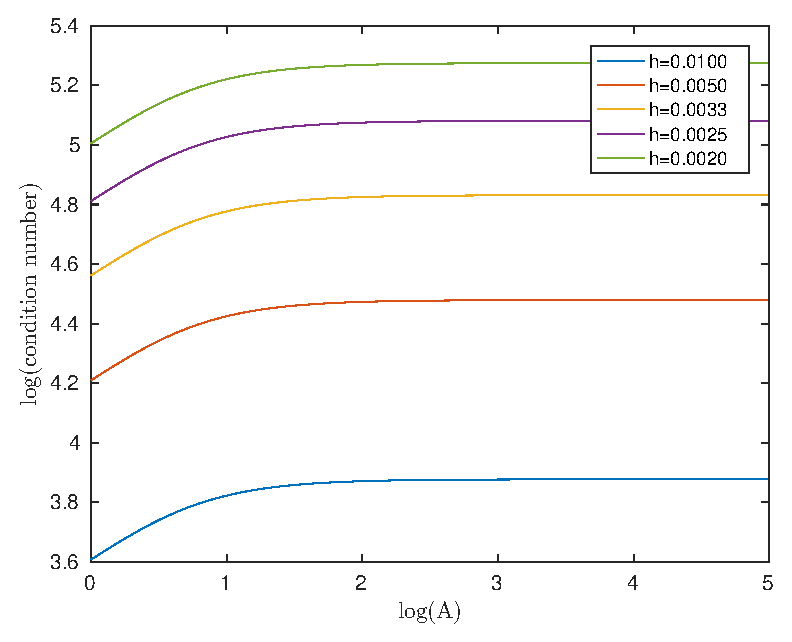
\includegraphics[width=\textwidth]{cond-A-pi-DD}
\caption{}
\end{subfigure}
\hfill
\begin{subfigure}{0.4\textwidth}
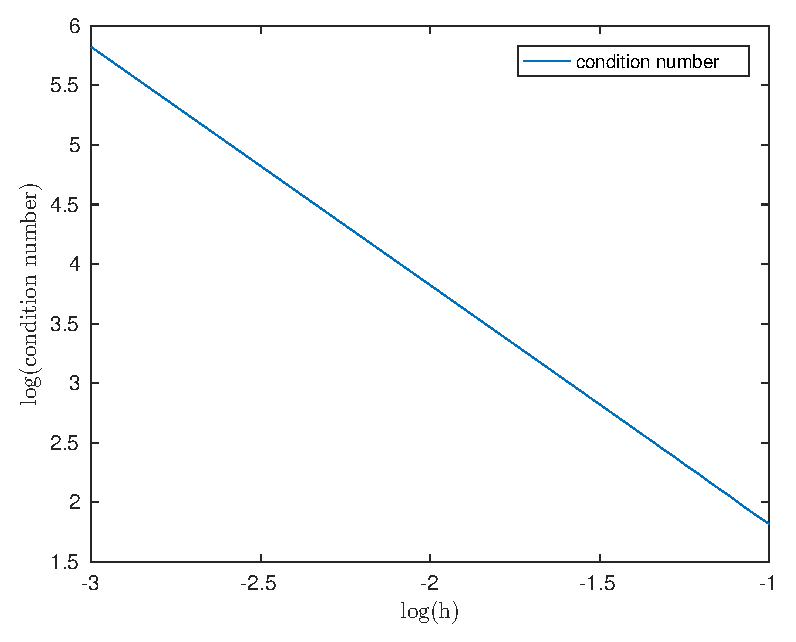
\includegraphics[width=\textwidth]{cond-N-pi-DD}
\caption{$A=10$}
\end{subfigure}
\caption{Scaled condition number, $\beta=\frac{1}{\pi}$, Dirichlet-Dirichlet boundary}
\end{figure}

\begin{figure}[h!]
\centering
\begin{subfigure}{0.4\textwidth}
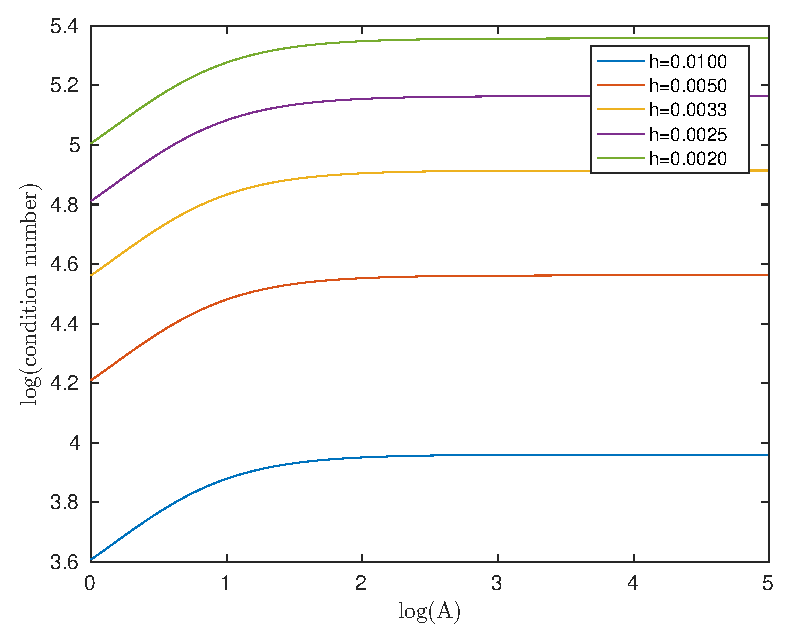
\includegraphics[width=\textwidth]{cond-A-4-DD}
\caption{}
\end{subfigure}
\hfill
\begin{subfigure}{0.4\textwidth}
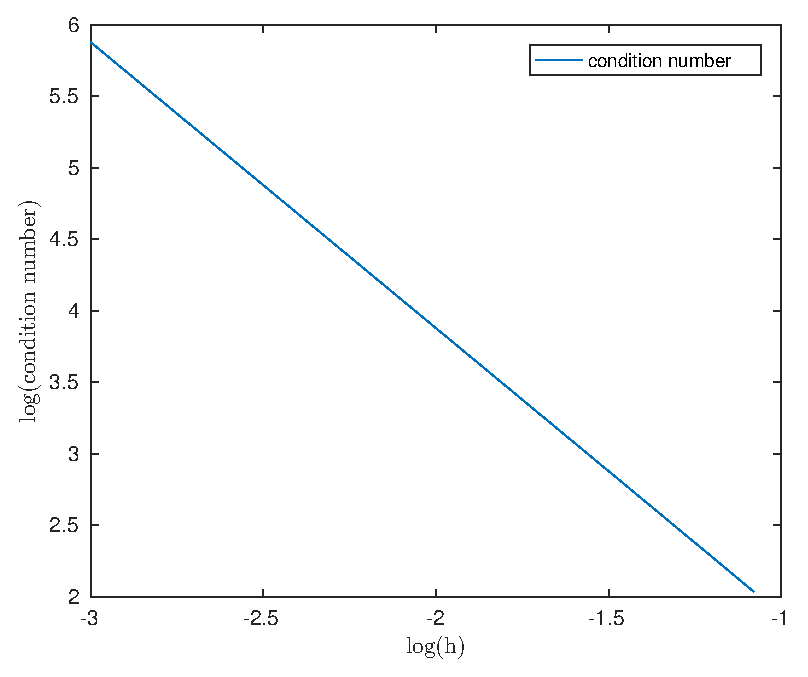
\includegraphics[width=\textwidth]{cond-N-4-DD}
\caption{$h=\frac{1}{4k},A=10$}
\end{subfigure}
\caption{Scaled condition number, $\beta=\frac{1}{4}$, Dirichlet-Dirichlet boundary}
\end{figure}

\begin{figure}[h!]
\centering
\begin{subfigure}{0.4\textwidth}
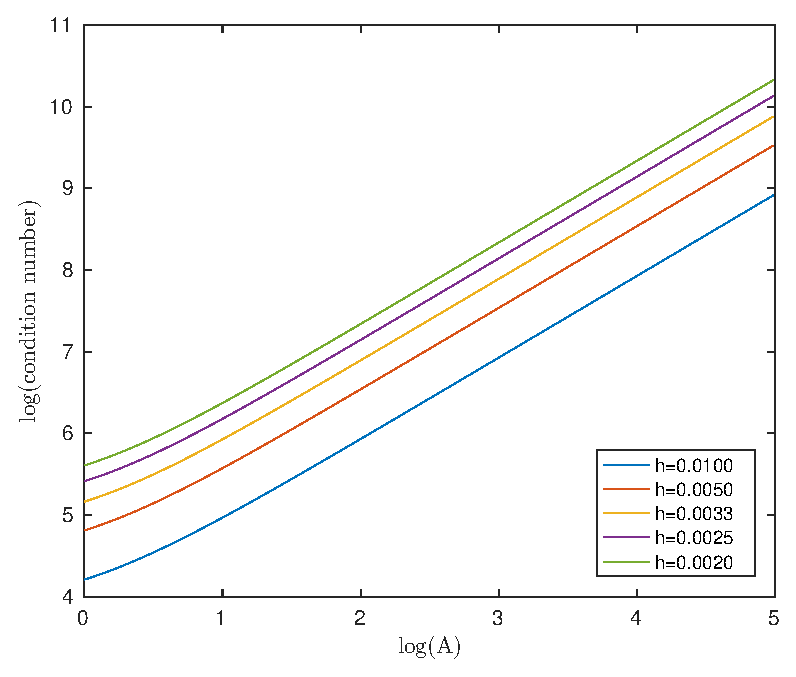
\includegraphics[width=\textwidth]{cond-A-pi-DN}
\caption{}
\end{subfigure}
\hfill
\begin{subfigure}{0.4\textwidth}
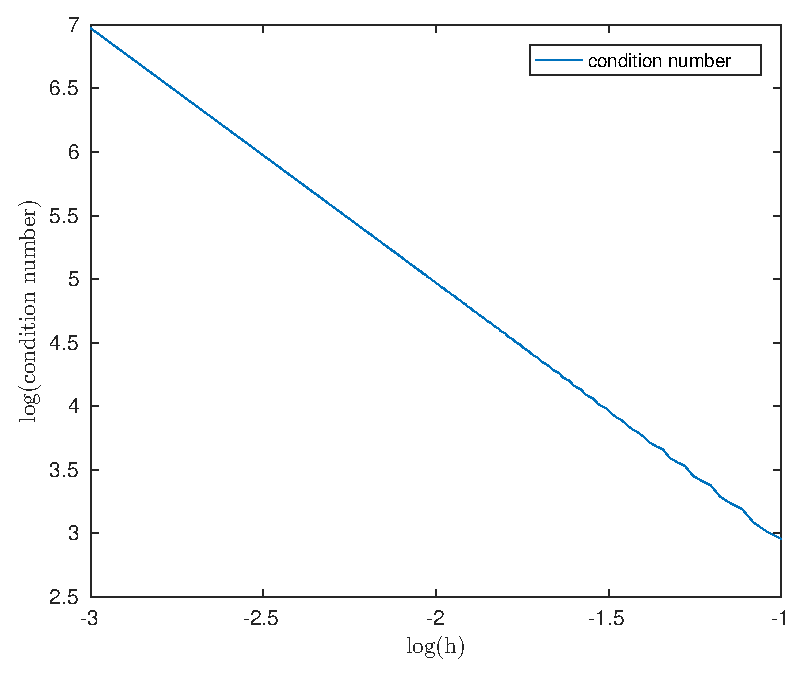
\includegraphics[width=\textwidth]{cond-N-pi-DN}
\caption{$A=10$}
\end{subfigure}
\caption{Scaled condition number, $\beta=\frac{1}{\pi}$, Dirichlet-Neumann boundary}
\end{figure}

\begin{figure}[h!]
\centering
\begin{subfigure}{0.4\textwidth}
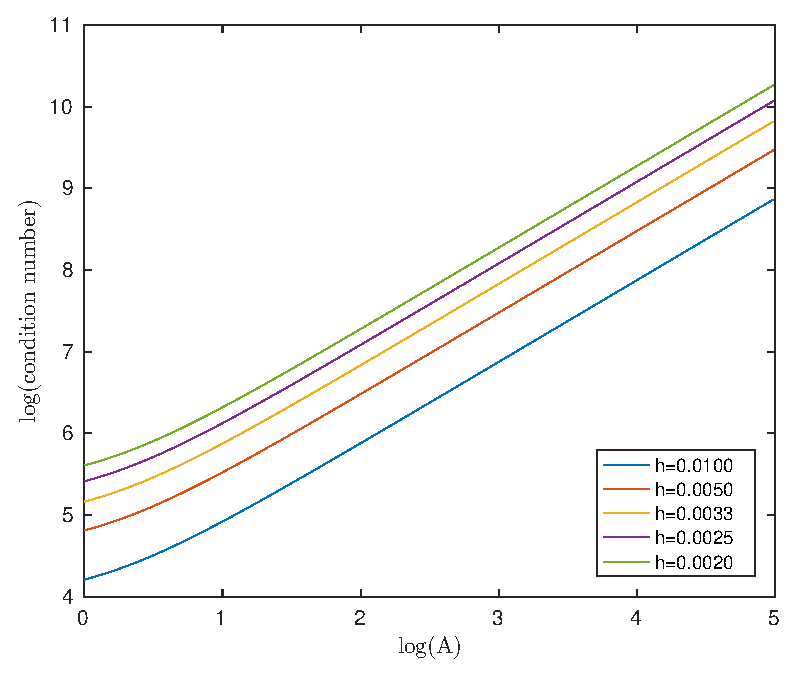
\includegraphics[width=\textwidth]{cond-A-4-DN}
\caption{}
\end{subfigure}
\hfill
\begin{subfigure}{0.4\textwidth}
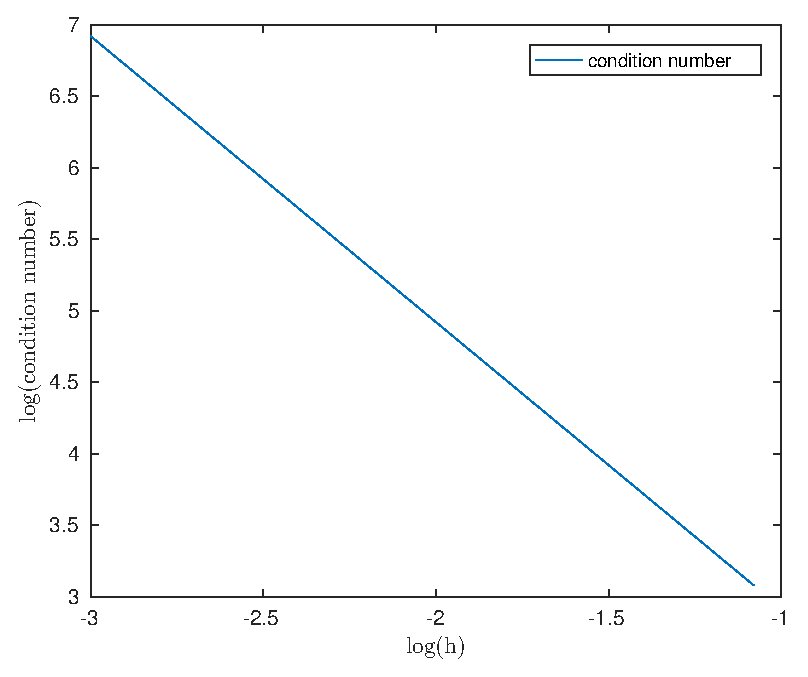
\includegraphics[width=\textwidth]{cond-N-4-DN}
\caption{$h=\frac{1}{4k},A=10$}
\end{subfigure}
\caption{Scaled condition number, $\beta=\frac{1}{4}$, Dirichlet-Neumann boundary}
\end{figure}

\begin{figure}[h!]
\centering
\begin{subfigure}{0.4\textwidth}
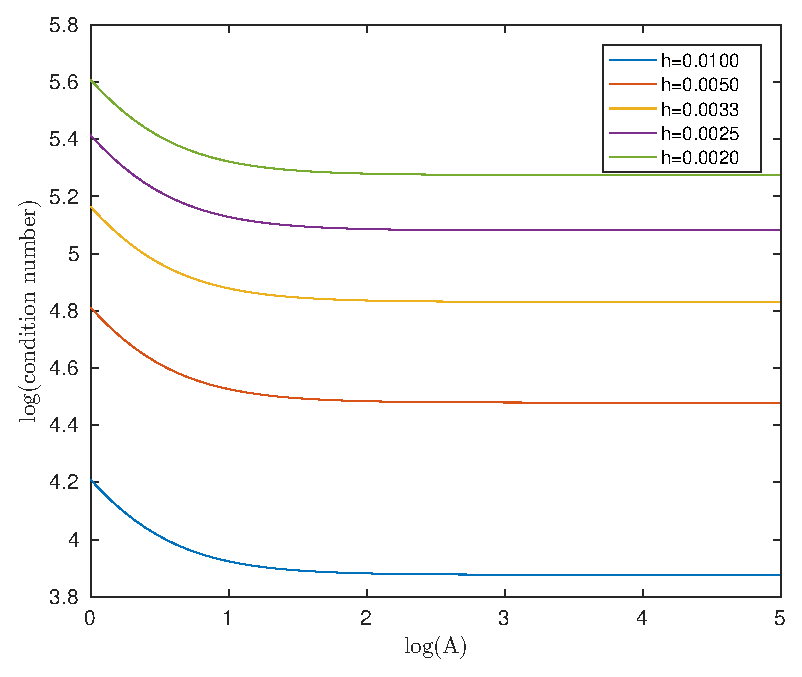
\includegraphics[width=\textwidth]{cond-A-pi-ND}
\caption{}
\end{subfigure}
\hfill
\begin{subfigure}{0.4\textwidth}
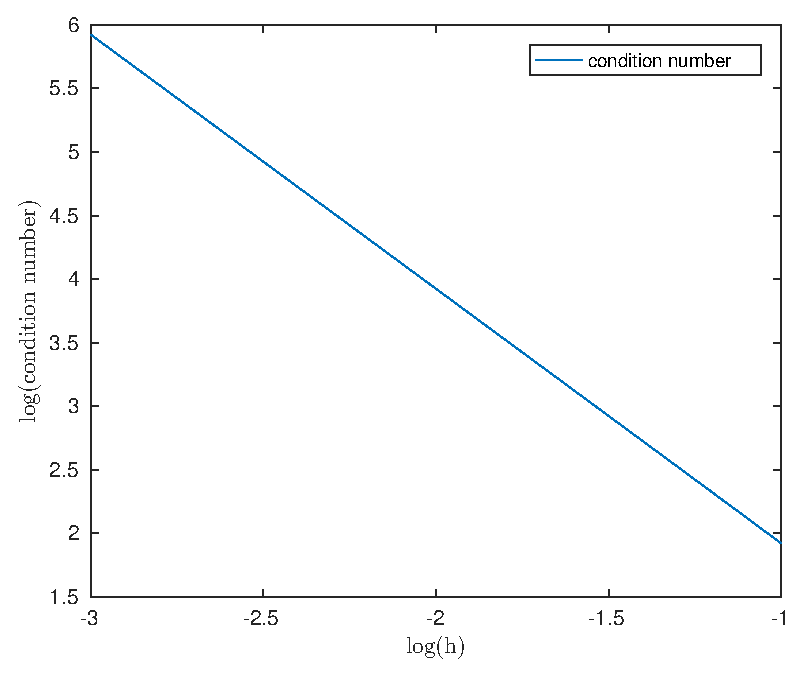
\includegraphics[width=\textwidth]{cond-N-pi-ND}
\caption{$A=10$}
\end{subfigure}
\caption{Scaled condition number, $\beta=\frac{1}{\pi}$, Neumann-Dirichlet boundary}
\end{figure}

\begin{figure}[h!]
\centering
\begin{subfigure}{0.4\textwidth}
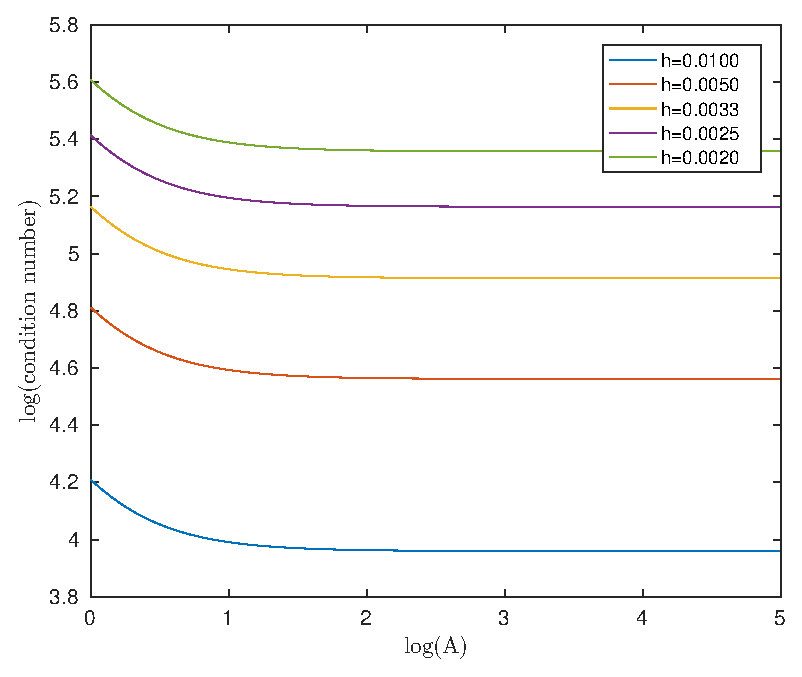
\includegraphics[width=\textwidth]{cond-A-4-ND}
\caption{}
\end{subfigure}
\hfill
\begin{subfigure}{0.4\textwidth}
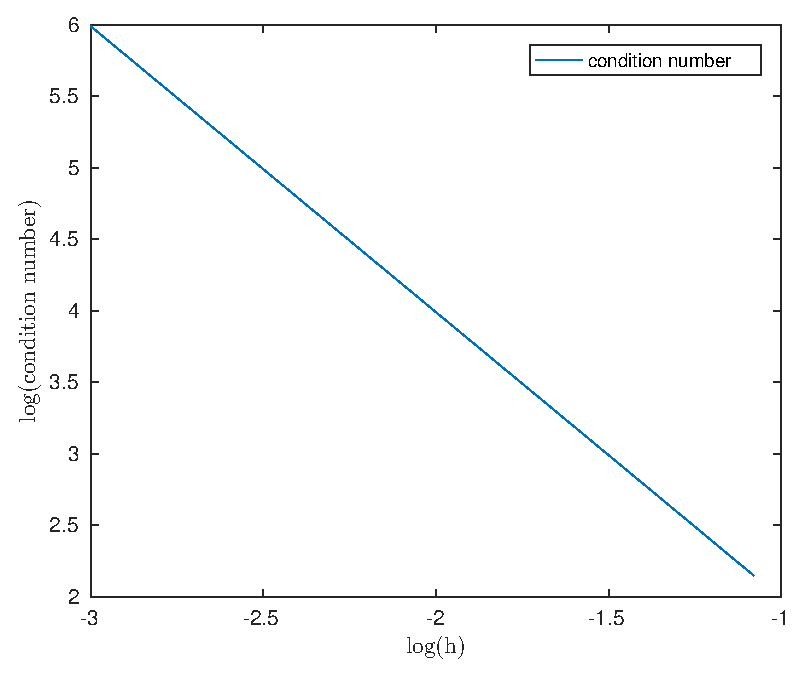
\includegraphics[width=\textwidth]{cond-N-4-ND}
\caption{$h=\frac{1}{4k},A=10$}
\end{subfigure}
\caption{Scaled condition number, $\beta=\frac{1}{4}$, Neumann-Dirichlet boundary}
\end{figure}

\subsection{Correction for error disturbance}
We know that the unbounded scaled condition number of the global stiffness matrix caused the disturbance in error of FEM solution. Below is a way to fix the disturbance.

Consider the global stiffness matrix and load vector in Dirichlet-Neumann boundary
\[
\textbf{K}=
\begin{bmatrix}
\frac{2}{h} & -\frac{1}{h} \\
-\frac{1}{h} & \frac{2}{h} & -\frac{1}{h} \\
& \ddots & \ddots & \ddots \\
&& -\frac{A}{h} & \frac{2A}{h} & -\frac{A}{h} \\
&&& -\frac{A}{h} & \frac{A}{h}
\end{bmatrix}
\quad \quad
\textbf{f}=
\begin{bmatrix}
h \\
h \\
\vdots \\
h \\
\frac{h}{2}
\end{bmatrix}
\]
impose Dirichlet boundary at $x=1$ and denote
\[
\textbf{A}=
\begin{bmatrix}
\frac{2}{h} & -\frac{1}{h} \\
-\frac{1}{h} & \frac{2}{h} & -\frac{1}{h} \\
& \ddots & \ddots & \ddots \\
&& -\frac{A}{h} & \frac{2A}{h} & -\frac{A}{h} \\
&&& -\frac{A}{h} & \frac{2A}{h}
\end{bmatrix}
\quad \quad
\textbf{b}=
\begin{bmatrix}
h \\
h \\
\vdots \\
h \\
h
\end{bmatrix}
\quad \quad
\textbf{c}=
\begin{bmatrix}
0 \\
0 \\
\vdots \\
0 \\
\frac{A}{h}
\end{bmatrix}
\]

Solve the systems
$$\textbf{Ax}=\textbf{b} \quad \quad \textbf{Az}=\textbf{c}$$
for $\textbf{x}$ and $\textbf{z}$, then the FEM solution
$$\textbf{u}_{h}=\textbf{x}+k\textbf{z}$$

Consider the energy. We know that for any $u$,
$$E(u)=B(u,u)-2\int_{0}^{1}f(x)u(x)dx$$
thus,
$$E(\textbf{u}_{h})=B(\textbf{x},\textbf{x})+2kB(\textbf{x},\textbf{z})+k^2B(\textbf{z},\textbf{z})-2\int_{0}^{1}f(x)\textbf{x}dx-2k\int_{0}^{1}f(x)\textbf{z}dx$$
to minimize energy, we take
$$\frac{\partial E(\textbf{u}_{h})}{\partial k}=0$$
therefore,
$$k=\frac{\int_{0}^{1}f(x)\textbf{z}dx-B(\textbf{x},\textbf{z})}{B(\textbf{z},\textbf{z})}$$

To compute, we use
$$B(\textbf{x},\textbf{x})=\sum_{i}\int_{\tau}a(x)(\frac{\textbf{x}_{i+1}-\textbf{x}_{i}}{h})^2dx=\sum_{i}a(x)\frac{(\textbf{x}_{i+1}-\textbf{x}_{i})^2}{h}$$
$$B(\textbf{z},\textbf{z})=\sum_{i}\int_{\tau}a(x)(\frac{\textbf{z}_{i+1}-\textbf{z}_{i}}{h})^2dx=\sum_{i}a(x)\frac{(\textbf{z}_{i+1}-\textbf{z}_{i})^2}{h}$$
$$B(\textbf{x},\textbf{z})=\sum_{i}\int_{\tau}a(x)\frac{(\textbf{x}_{i+1}-\textbf{x}_{i})(\textbf{z}_{i+1}-\textbf{z}_{i})}{h^2}dx=\sum_{i}a(x)\frac{(\textbf{x}_{i+1}-\textbf{x}_{i})(\textbf{z}_{i+1}-\textbf{z}_{i})}{h}$$
$$\int_{0}^{1}f(x)\textbf{x}dx=\sum_{i}\frac{h(\textbf{x}_{i+1}-\textbf{x}_{i})}{2}$$
$$\int_{0}^{1}f(x)\textbf{z}dx=\sum_{i}\frac{h(\textbf{z}_{i+1}-\textbf{z}_{i})}{2}$$

The energy difference $E(\textbf{u}_{h})-E(u)$ is computed as opposed to error in energy norm. Here $u$ is the exact solution. As illustrated by the graphs, disturbance of error for Dirichlet-Neumann problem vanished.

\begin{figure}[h!]
\centering
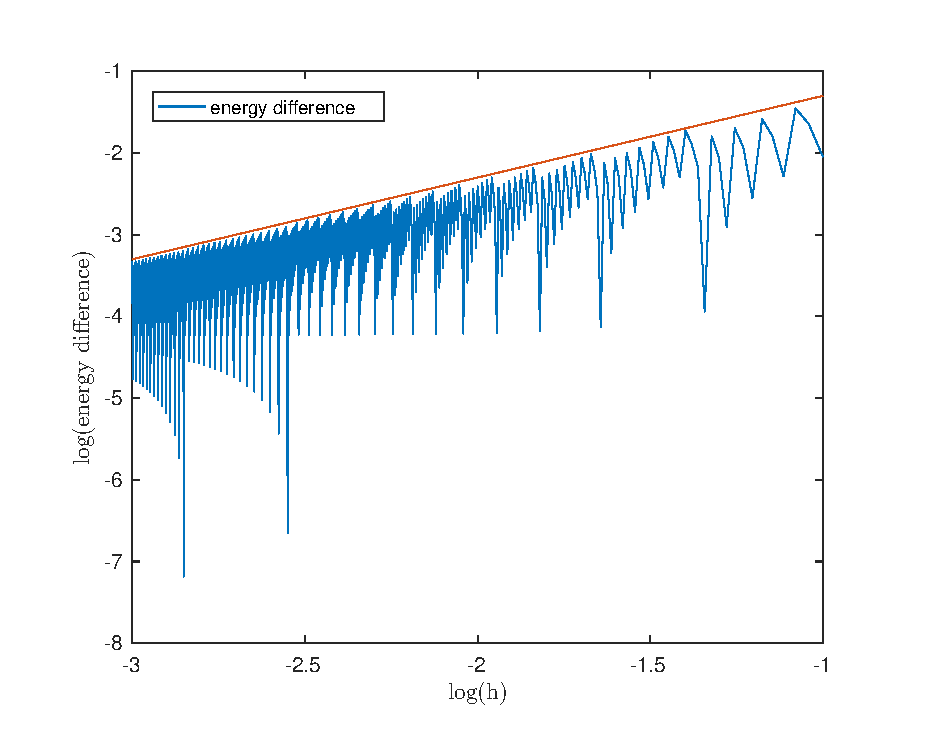
\includegraphics[scale=0.7]{energy-pi}
\caption{Energy Difference, $\beta=\frac{1}{\pi},A=10^{12}$, Dirichlet-Neumann boundary}
\end{figure}
\pagebreak
\begin{figure}[h!]
\centering
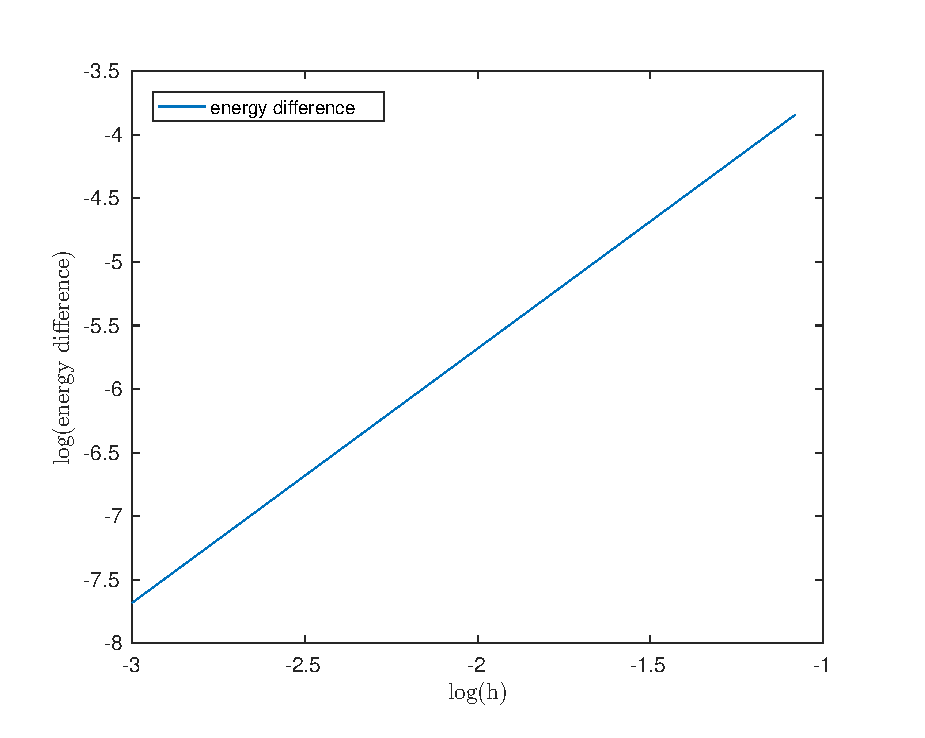
\includegraphics[scale=0.7]{energy-4}
\caption{Energy Difference, $h=\frac{1}{4k},\beta=\frac{1}{4},A=10^{12}$, Dirichlet-Neumann boundary}
\end{figure}

\subsection{Position of the constraint}
So far the constraint of the global stiffness matrix is on the endpoints, i.e. $x=0$ or $x=1$. The constraint can also be imposed elsewhere. We consider a Neumann-Neumann boundary problem with constraint put somewhere other than the endpoints.

Still consider the scaled global stiffness matrix for interface $\beta=\frac{1}{4}$
\[
\lim_{A \to \infty}\textbf{K}^{*}=
\begin{bmatrix}
1 & -\frac{1}{\sqrt{2}} \\
-\frac{1}{\sqrt{2}} & 1 & -\frac{1}{2} \\
& \ddots & \ddots & \ddots \\
&& -\frac{1}{2} & 1 \\
&&& & 1 & -\frac{1}{\sqrt{2}} \\
&&&& -\frac{1}{\sqrt{2}} & 1 & -\frac{1}{2} \\
&&&&& \ddots & \ddots & \ddots \\
&&&&&& -\frac{1}{2} & 1 & -\frac{1}{\sqrt{2}} \\
&&&&&&& -\frac{1}{\sqrt{2}} & 1
\end{bmatrix}
\quad \quad
\textbf{K}^{*}_{A \to \infty}=
\left[
\begin{array}{c|c}
\textbf{K}^{*}_{1} & \\
\hline
& \textbf{K}^{*}_{2}
\end{array}
\right]
\]
if we put the constraint right on the interface, i.e. at $x=\frac{1}{4}$, then the scaled condition number is bounded. If we put the constraint in $\textbf{K}^{*}_{1}$, i.e. at $x=0.1$, then the problem is analog to a Dirichlet-Neumann problem; and if we put the constraint in $\textbf{K}^{*}_{2}$, i.e. at $x=0.9$, then the problem will become a Neumann-Dirichlet problem.

\begin{figure}[h!]
\centering
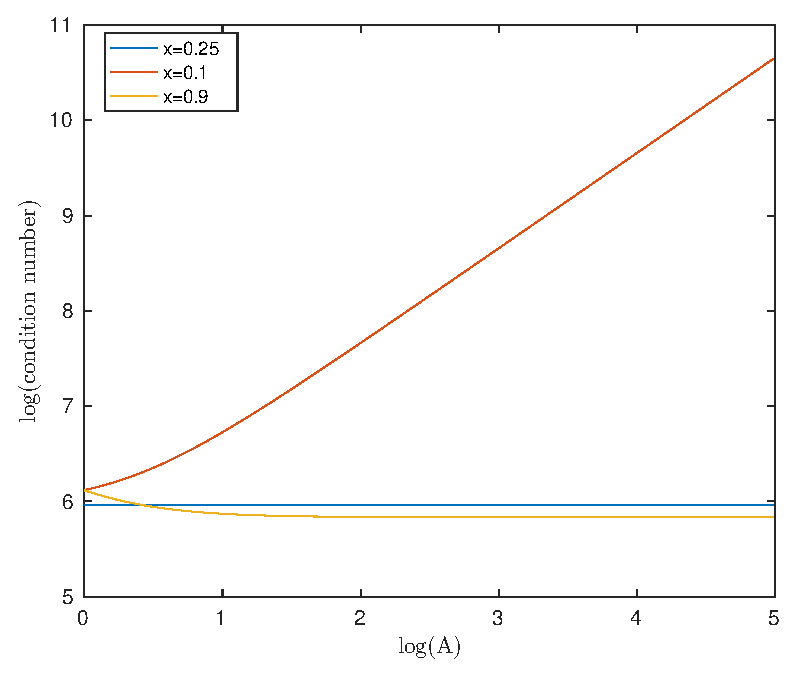
\includegraphics[scale=0.7]{cond-A-4-NN}
\caption{Scaled condition number, $h=10^{-3},\beta=\frac{1}{4}$, Neumann-Neumann boundary}
\end{figure}

The result is similar for interface $\beta=\frac{1}{\pi}$. But instead of putting the constraint on the interface, we put it near the interface, i.e. at $x_{i}$ or $x_{i+1}$. \\
\setlength{\unitlength}{1cm}
\thicklines
\begin{picture}(0,2.5)(-7,0)
\put(0,1){\line(1,0){4}}
\put(2,0){\line(0,1){2}}
\put(1.5,1){\line(0,1){0.1}}
\put(2.5,1){\line(0,1){0.1}}
\put(-0.1,0.7){$x_{1}$}
\put(1.4,0.7){$x_{i}$}
\put(2.2,0.7){$x_{i+1}$}
\put(3.6,0.7){$x_{n+1}$}
\put(2.1,0){$\beta$}
\end{picture}

\begin{figure}[h!]
\centering
\begin{subfigure}{0.4\textwidth}
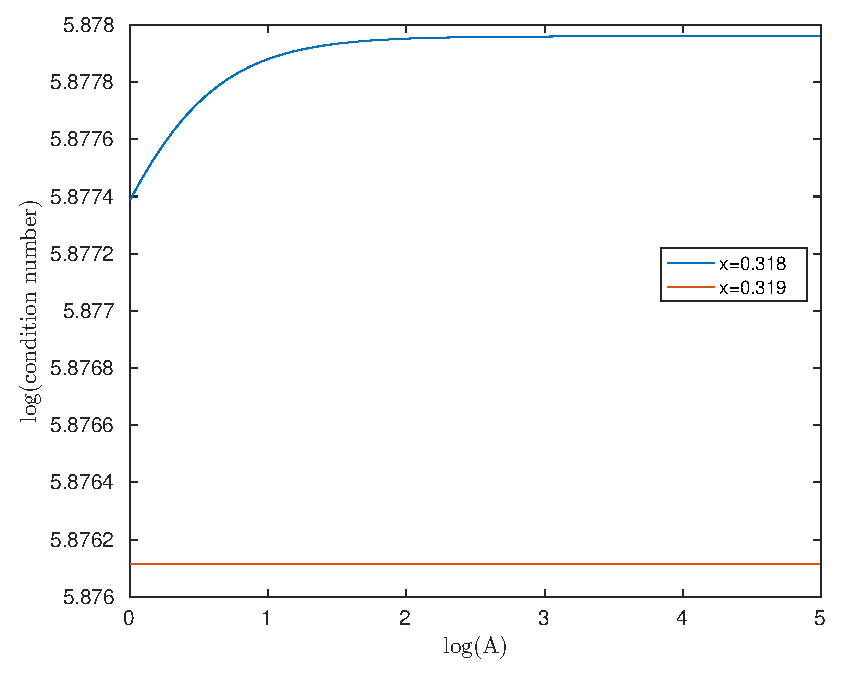
\includegraphics[width=\textwidth]{cond-A-pi-NN-near}
\caption{Constraint near the interface}
\end{subfigure}
\hfill
\begin{subfigure}{0.4\textwidth}
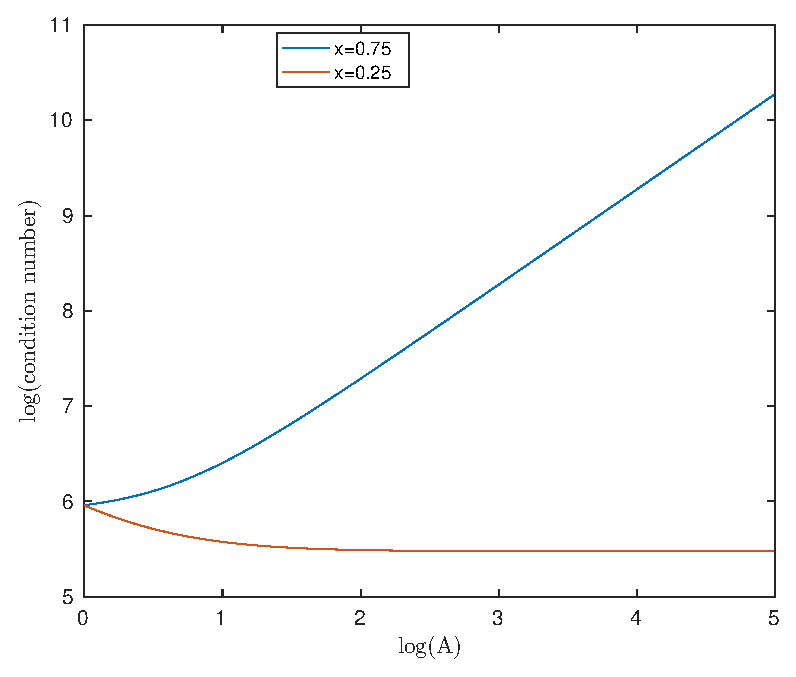
\includegraphics[width=\textwidth]{cond-A-pi-NN-away}
\caption{Constraint away from the interface}
\end{subfigure}
\caption{Scaled condition number, $h=10^{-3},\beta=\frac{1}{\pi}$, Neumann-Neumann boundary}
\end{figure}

\subsection{Multiple interfaces}
Consider a uniform mesh on $[0,1]$ with two interfaces, $\beta_{1}=\frac{1}{4}$ and $\beta_{2}=\frac{3}{4}$ \\
\setlength{\unitlength}{1cm}
\thicklines
\begin{picture}(0,2.5)(-7,0)
\put(0,1){\line(1,0){4}}
\put(1,0){\line(0,1){2}}
\put(3,0){\line(0,1){2}}
\put(1.1,0){$\beta_{1}$}
\put(3.1,0){$\beta_{2}$}
\put(0.4,1.1){$1$}
\put(1.9,1.1){$A$}
\put(3.4,1.1){$1$} 
\end{picture}

As before, we first scale the global stiffness matrix and then let the contrast $A$ goes to infinity. We obtain
\[
\lim_{A \to \infty}\textbf{K}^{*}= \\
\begin{bmatrix}
1 & -\frac{1}{\sqrt{2}} \\
& \ddots & \ddots \\
& -\frac{1}{2} & 1 \\
&&& 1 & -\frac{1}{\sqrt{2}} \\
&&&& \ddots & \ddots \\
&&&& -\frac{1}{2} & 1 \\
&&&&&& 1 & -\frac{1}{2} \\
&&&&&&& \ddots & \ddots \\
&&&&&&& -\frac{1}{2} & 1
\end{bmatrix}
\]

Similar to the case with one interface, the scaled global stiffness matrix is divided into three completely separated sub-matrices \\
\[
\textbf{K}^{*}_{A \to \infty}=
\left[
\begin{array}{c|c|c}
\textbf{K}^{*}_{1} & \\
\hline
& \textbf{K}^{*}_{2} \\
\hline
&& \textbf{K}^{*}_{3}
\end{array}
\right]
\]

In this case, if we only put constraints on the endpoints $x=0$ and  $x=1$, the sub-matrix $\textbf{K}^{*}_{2}$ will always be a Neumann-Neumann problem, and thus the scaled condition number of $\textbf{K}^{*}_{2}$ is unbounded, and hence the scaled condition number of the global stiffness matrix goes to infinity, as illustrated by the following graphs.

\begin{figure}[h!]
\centering
\begin{subfigure}{0.4\textwidth}
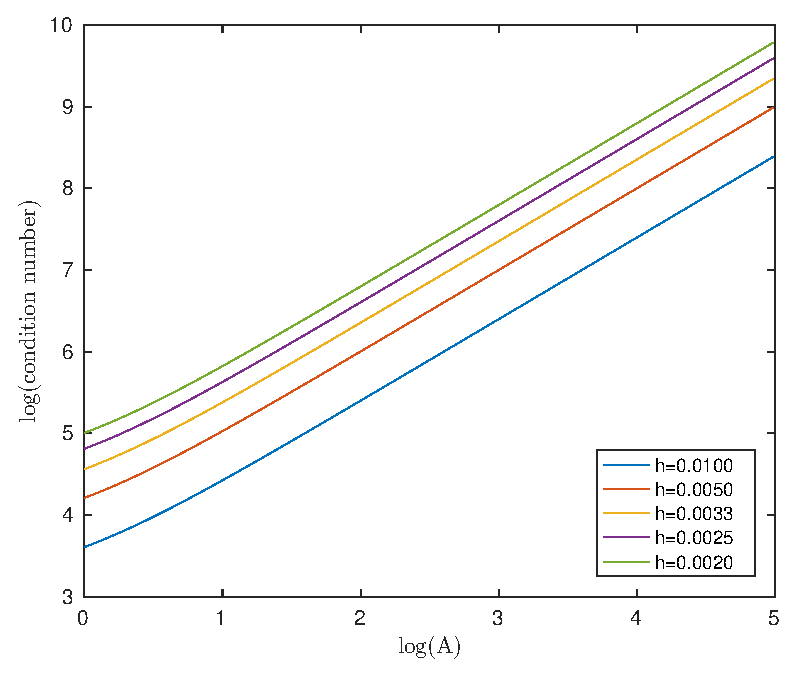
\includegraphics[width=\textwidth]{cond-A-42-DD}
\caption{Dirichlet-Dirichlet boundary}
\end{subfigure}
\hfill
\begin{subfigure}{0.4\textwidth}
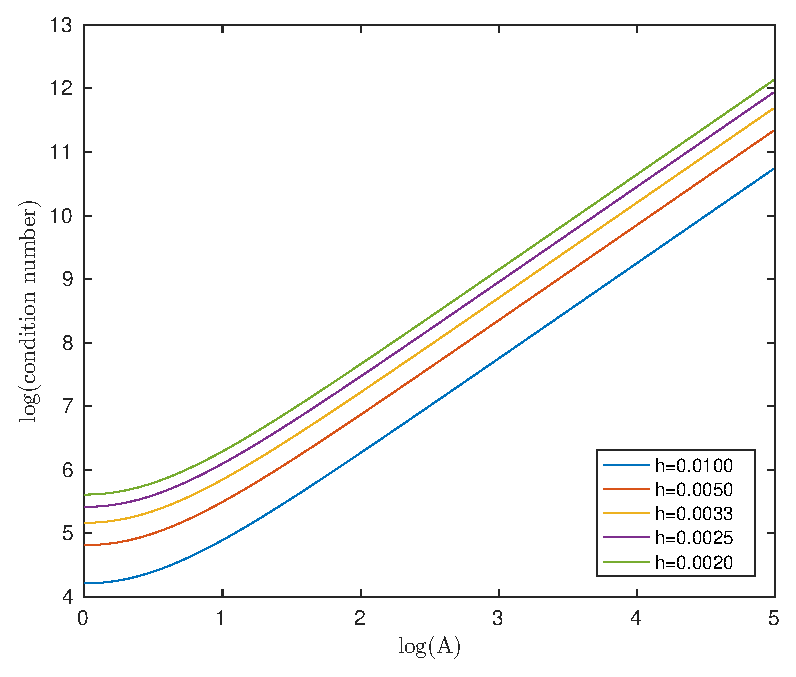
\includegraphics[width=\textwidth]{cond-A-42-DN}
\caption{Dirichlet-Neumann boundary}
\end{subfigure}
\vfill
\begin{subfigure}{0.4\textwidth}
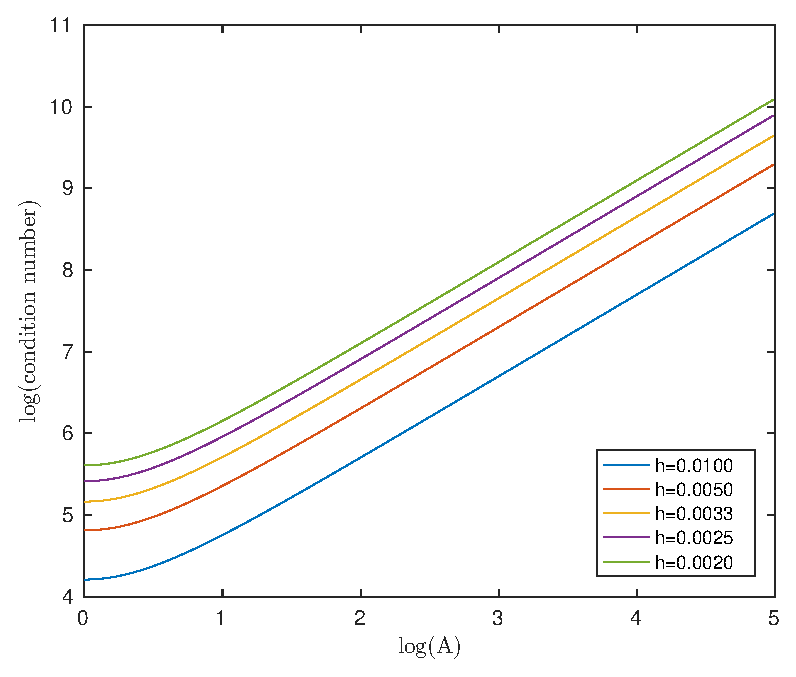
\includegraphics[width=\textwidth]{cond-A-42-ND}
\caption{Neumann-Dirichlet boundary}
\end{subfigure}
\caption{Scaled condition number, $\beta_{1}=\frac{1}{4}$, $\beta_{2}=\frac{3}{4}$}
\end{figure}
\pagebreak
If we put constraints on the endpoints ($x=0$ and $x=1$), either Dirichlet or Neumann, then an additional constraint has to be imposed at $\beta_{1}=\frac{1}{4}$ in order to obtain an analog with previous problems. 

To obtain a bounded scaled condition number, we need to put an additional constraint on one of the interfaces. In the following graph, constraints are put on both the endpoints and on one of the interfaces, i.e. $x=0$, $x=1$, and $x=\frac{1}{4}$.
\pagebreak
\begin{figure}[h!]
\centering
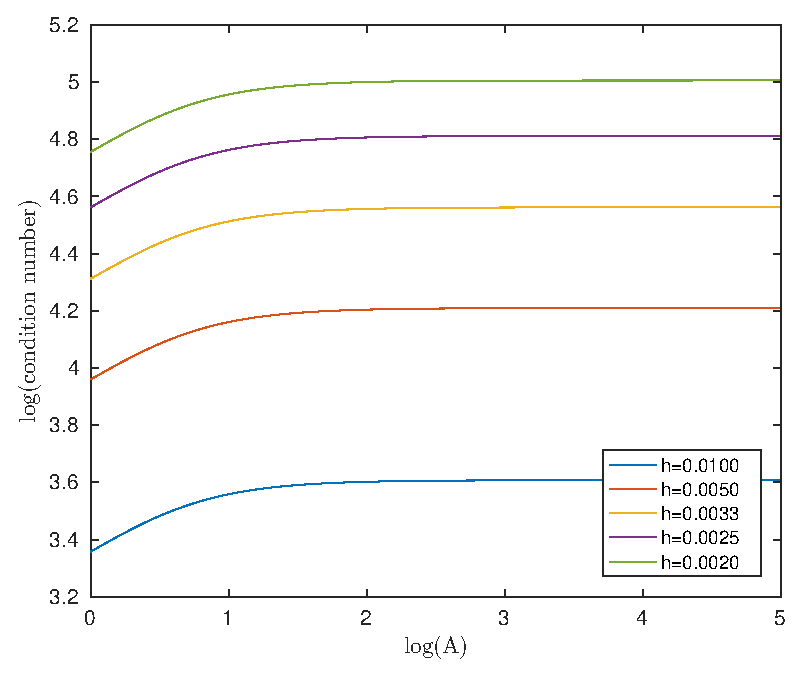
\includegraphics[scale=0.7]{cond-A-42-NN}
\caption{Scaled condition number, $\beta_{1}=\frac{1}{4}$, $\beta_{2}=\frac{3}{4}$}
\end{figure}

\section{Two-dimensional interface problem}
\subsection{Construction of global stiffness matrix}
Consider a uniform mesh on $\Omega=[0,1]\times [0,1]$ \\
\setlength{\unitlength}{1cm}
\thicklines
\begin{picture}(0,5.5)(-7,0.5)
\multiput(0,1)(0,1){5}{\line(1,0){4}}
\multiput(0,1)(1,0){5}{\line(0,1){4}}
\put(0,5){\line(1,-1){4}}
\put(0,4){\line(1,-1){3}}
\put(0,3){\line(1,-1){2}}
\put(0,2){\line(1,-1){1}}
\put(1,5){\line(1,-1){3}}
\put(2,5){\line(1,-1){2}}
\put(3,5){\line(1,-1){1}}
\put(-0.1,0.65){$1$}
\put(0.9,0.65){$2$}
\put(1.9,0.65){$3$}
\put(2.9,0.65){$4$}
\put(3.9,0.65){$5$}
\put(-0.3,1.9){$6$}
\put(4.1,1.9){$10$}
\put(-0.5,2.9){$11$}
\put(4.1,2.9){$15$}
\put(-0.5,3.9){$16$}
\put(4.1,3.9){$20$}
\put(-0.2,5.1){$21$}
\put(0.8,5.1){$22$}
\put(1.8,5.1){$23$}
\put(2.8,5.1){$24$}
\put(3.8,5.1){$25$}
\end{picture} \\
In this case, the region $\Omega$ is divided into $32$ elements and $25$ nodal points, with $h=0.2$.
The boundary $\partial \Omega$ is the boundary of the square, namely \\
\[
\partial \Omega=
\begin{cases}
x=0 & 0 \leq y \leq 1 \\
x=1 & 0 \leq y \leq 1 \\
y=0 & 0 \leq x \leq 1 \\
y=1 & 0 \leq x \leq 1
\end{cases}
\] \\
In theory, we should put Dirichlet or Neumann boundary on all the points on $\partial \Omega$, but in order to show the growth of the scaled condition number, several points are enough.

Consider a master element on $\Omega$ \\
\setlength{\unitlength}{1cm}
\thicklines
\begin{picture}(0,2.5)(-8,0)
\put(0,0){\vector(1,0){2}}
\put(0,0){\vector(0,1){2}}
\put(0,1.5){\line(1,-1){1.5}}
\put(-0.2,-0.35){\footnotesize$A$}
\put(1.3,-0.35){\footnotesize$B$}
\put(-0.35,1.3){\footnotesize$C$}
\put(0.4,0.3){$\tau$}
\end{picture} \\
where
$$N_{A}=1-x-y$$
$$N_{B}=x$$
$$N_{C}=y$$

Obviously,
$$N_{A}N_{A}=\iint_{\tau}(\frac{\partial N_{A}}{\partial x})^2+(\frac{\partial N_{A}}{\partial y})^2dA=1$$
$$N_{A}N_{B}=\iint_{\tau}\frac{\partial N_{A}}{\partial x}\frac{\partial N_{B}}{\partial x}+\frac{\partial N_{A}}{\partial y}\frac{\partial N_{B}}{\partial y}dA=-\frac{1}{2}$$
Similarly, compute all the other values $N_{A}N_{C}=-\frac{1}{2}$, $N_{B}N_{A}=-\frac{1}{2}$, $N_{B}N_{B}=\frac{1}{2}$, $N_{B}N_{C}=0$, $N_{C}N_{A}=-\frac{1}{2}$, $N_{C}N_{B}=0$, and $N_{C}N_{C}=\frac{1}{2}$.

Thus, we can construct the local stiffness matrix
\[
\begin{bmatrix}
1 & -\frac{1}{2} & -\frac{1}{2} \\
-\frac{1}{2} & \frac{1}{2} & 0 \\
-\frac{1}{2} & 0 & \frac{1}{2}
\end{bmatrix}
\]
From here, it is easy to construct the global stiffness matrix (see reference 1 for more details).

\subsection{Linear interface}
Consider a uniform mesh on $\Omega$ with a linear interface $\beta=\frac{1}{4}$. We take $a(x,y)=1$ when $(x,y)$ is on the left of the interface (excluding); and $a(x,y)=A$ otherwise. \\
\setlength{\unitlength}{1cm}
\thicklines
\begin{picture}(0,6)(-7,0.5)
\put(0,1){\vector(1,0){5}}
\put(0,1){\vector(0,1){5}}
\multiput(0,1)(0,1){5}{\line(1,0){4}}
\multiput(0,1)(1,0){5}{\line(0,1){4}}
\put(0,5){\line(1,-1){4}}
\put(0,4){\line(1,-1){3}}
\put(0,3){\line(1,-1){2}}
\put(0,2){\line(1,-1){1}}
\put(1,5){\line(1,-1){3}}
\put(2,5){\line(1,-1){2}}
\put(3,5){\line(1,-1){1}}
\linethickness{1mm}
\put(1,1){\line(0,1){4}}
\put(5,0.7){$x$}
\put(-0.25,6){$y$}
\put(-0.1,0.65){$1$}
\put(0.9,0.65){$2$}
\put(1.9,0.65){$3$}
\put(2.9,0.65){$4$}
\put(3.9,0.65){$5$}
\put(-0.3,1.9){$6$}
\put(4.1,1.9){$10$}
\put(-0.5,2.9){$11$}
\put(4.1,2.9){$15$}
\put(-0.5,3.9){$16$}
\put(4.1,3.9){$20$}
\put(-0.5,5.1){$21$}
\put(0.8,5.1){$22$}
\put(1.8,5.1){$23$}
\put(2.8,5.1){$24$}
\put(3.8,5.1){$25$}
\end{picture}

Like in one-dimensional problem, we consider the scaled condition number of the global stiffness matrix. First we put Neumann boundary on all $\partial \Omega$, i.e. nodal points 1, 2, 3, 4, 5, 6, 10, 11, 15, 16, 20, 21, 22, 23, 24, 25 in the above figure. Then we impose constraints on some points. By saying Dirichlet-Dirichlet boundary, we mean putting constraints on  points $(0,0)$ and $(1,1)$. Likewise, we put a constraint on point $(0,0)$ to simulate Dirichlet-Neumann boundary, and we put a constraint on point $(1,1)$ to simulate Neumann-Dirichlet boundary.

As we can see in the following figure, the two-dimensional problem is a complete analog to the one-dimensional problem. Also, in order to obtain a bounded scaled condition number, we can put the constraint on the interface (only one point is enough).
\pagebreak
\begin{figure}[h!]
\centering
\begin{subfigure}{0.4\textwidth}
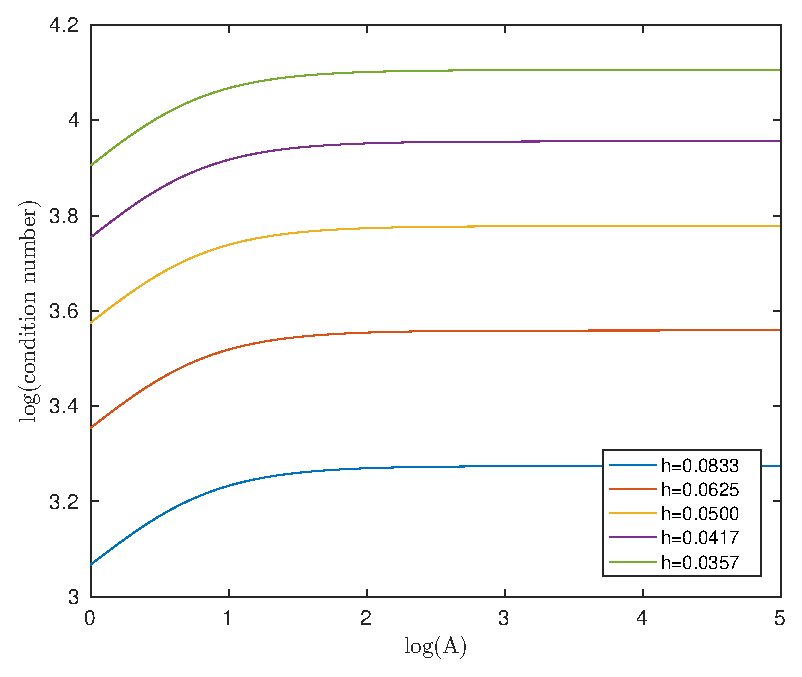
\includegraphics[width=\textwidth]{cond-A-2D-linear-DD}
\caption{Dirichlet-Dirichlet boundary}
\end{subfigure}
\hfill
\begin{subfigure}{0.4\textwidth}
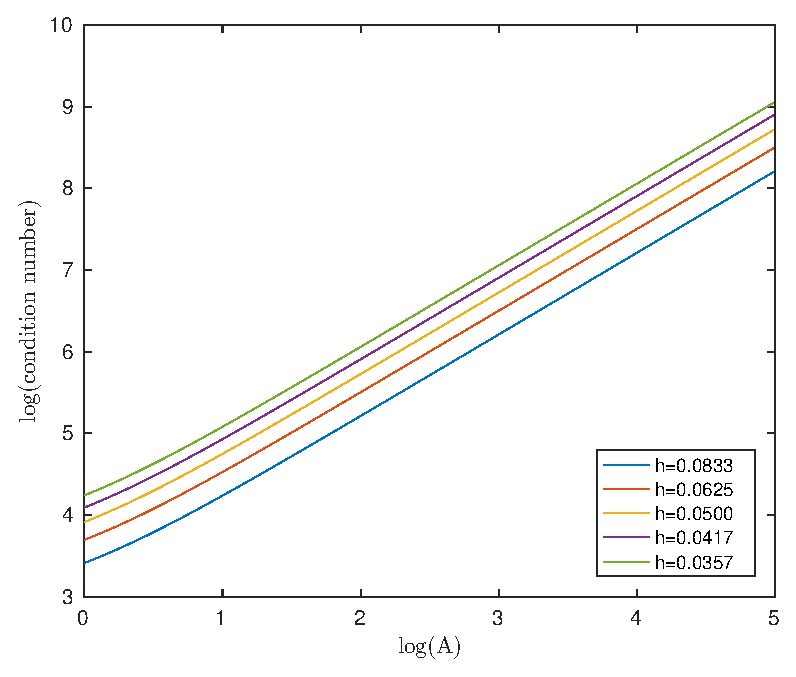
\includegraphics[width=\textwidth]{cond-A-2D-linear-DN}
\caption{Dirichlet-Neumann boundary}
\end{subfigure}
\vfill
\begin{subfigure}{0.4\textwidth}
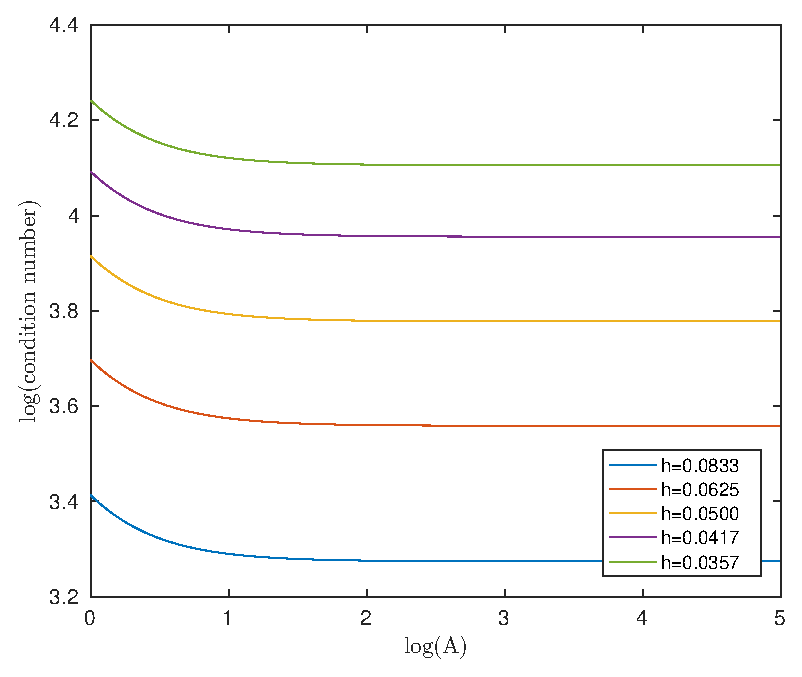
\includegraphics[width=\textwidth]{cond-A-2D-linear-ND}
\caption{Neumann-Dirichlet boundary}
\end{subfigure}
\hfill
\begin{subfigure}{0.4\textwidth}
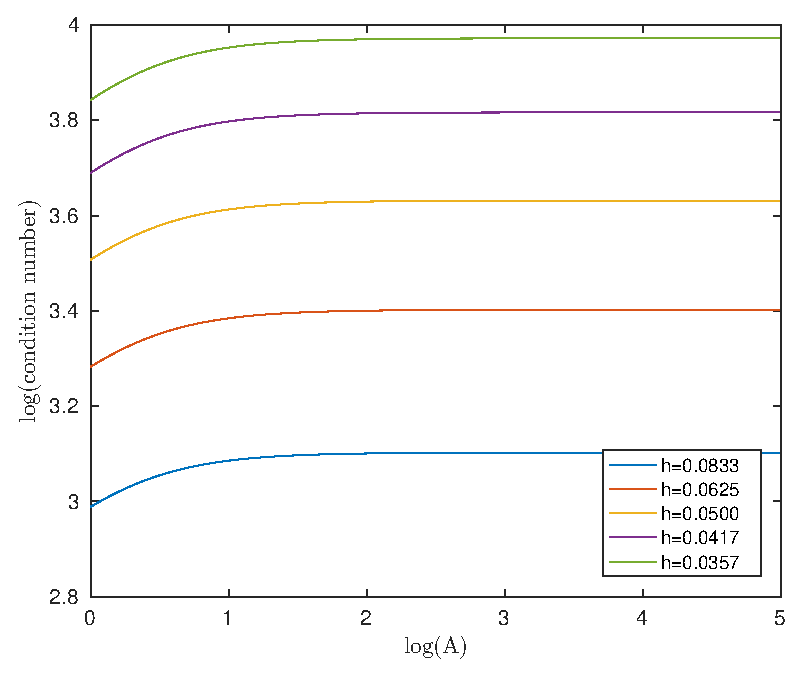
\includegraphics[width=\textwidth]{cond-A-2D-linear-interface}
\caption{Constraint on $(\frac{1}{4}, \frac{1}{4})$}
\end{subfigure}
\caption{Scaled condition number, linear interface $\beta=\frac{1}{4}$}
\end{figure}

Likewise, consider a pseudo-linear interface where there is a distortion in the middle of $\beta$. \\
\setlength{\unitlength}{1cm}
\thicklines
\begin{picture}(0,6.5)(-6.5,0)
\put(0,0){\vector(1,0){6}}
\put(0,0){\vector(0,1){6}}
\multiput(0,0)(0,1){6}{\line(1,0){5}}
\multiput(0,0)(1,0){6}{\line(0,1){5}}
\put(0,5){\line(1,-1){5}}
\put(0,4){\line(1,-1){4}}
\put(0,3){\line(1,-1){3}}
\put(0,2){\line(1,-1){2}}
\put(0,1){\line(1,-1){1}}
\put(1,5){\line(1,-1){4}}
\put(2,5){\line(1,-1){3}}
\put(3,5){\line(1,-1){2}}
\put(4,5){\line(1,-1){1}}
\linethickness{1mm}
\put(2,0){\line(0,1){2}}
\put(2,2){\line(-1,0){1}}
\put(1,2){\line(0,1){1}}
\put(1,3){\line(1,0){1}}
\put(2,3){\line(0,1){2}}
\put(6,-0.3){$x$}
\put(-0.3,6){$y$}
\end{picture}

Still, we consider the scaled condition number of the global stiffness matrix.
\pagebreak
\begin{figure}[h!]
\centering
\begin{subfigure}{0.4\textwidth}
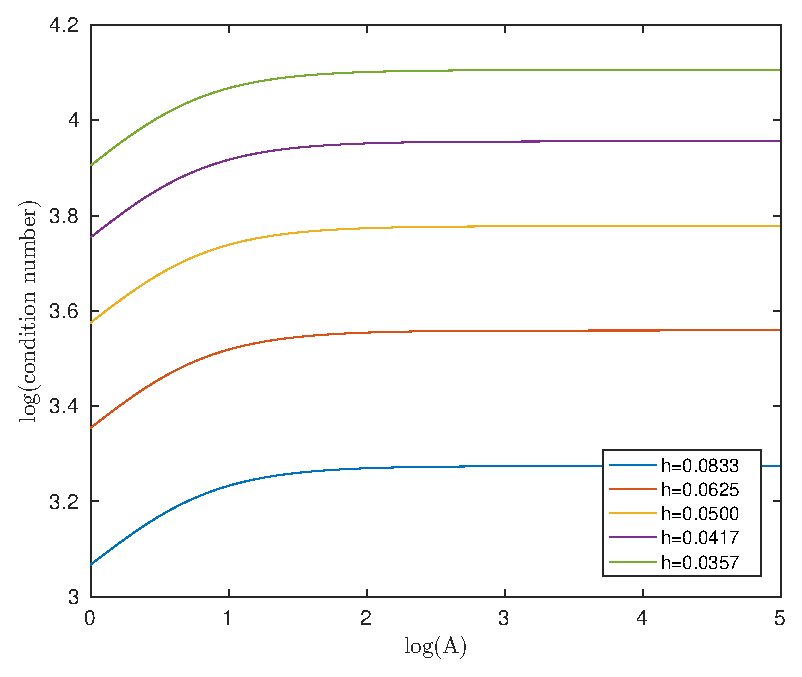
\includegraphics[width=\textwidth]{cond-A-2D-plinear-DD}
\caption{Dirichlet-Dirichlet boundary}
\end{subfigure}
\hfill
\begin{subfigure}{0.4\textwidth}
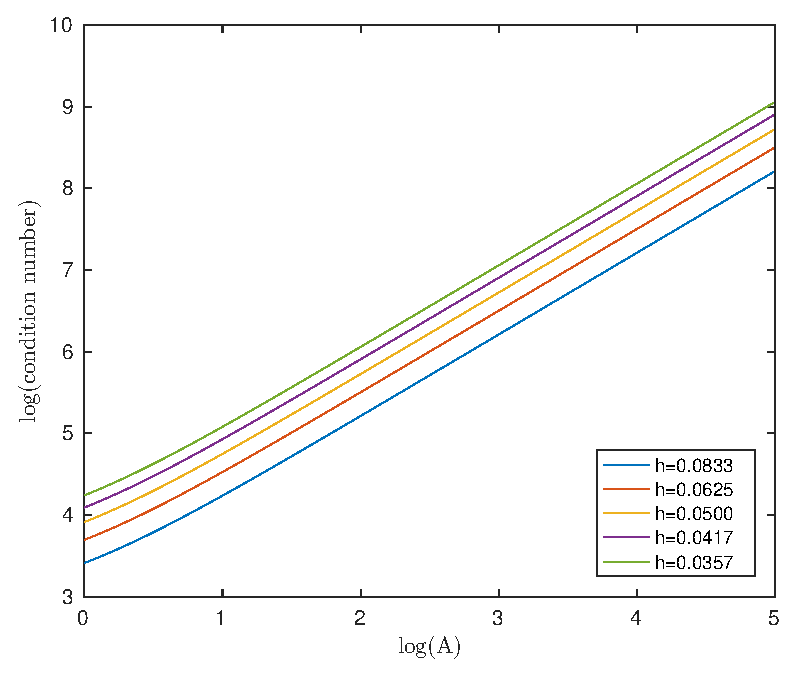
\includegraphics[width=\textwidth]{cond-A-2D-plinear-DN}
\caption{Dirichlet-Neumann boundary}
\end{subfigure}
\vfill
\begin{subfigure}{0.4\textwidth}
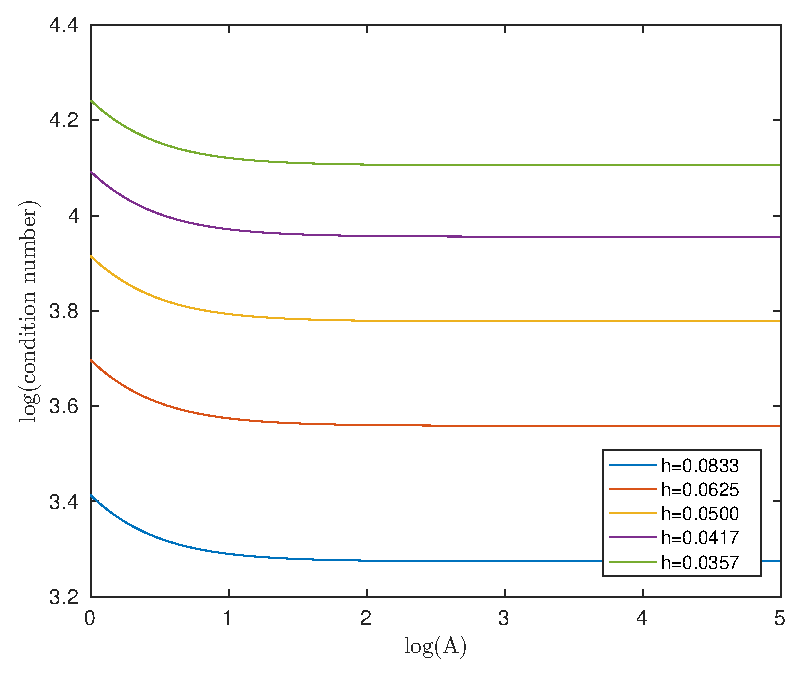
\includegraphics[width=\textwidth]{cond-A-2D-plinear-ND}
\caption{Neumann-Dirichlet boundary}
\end{subfigure}
\hfill
\begin{subfigure}{0.4\textwidth}
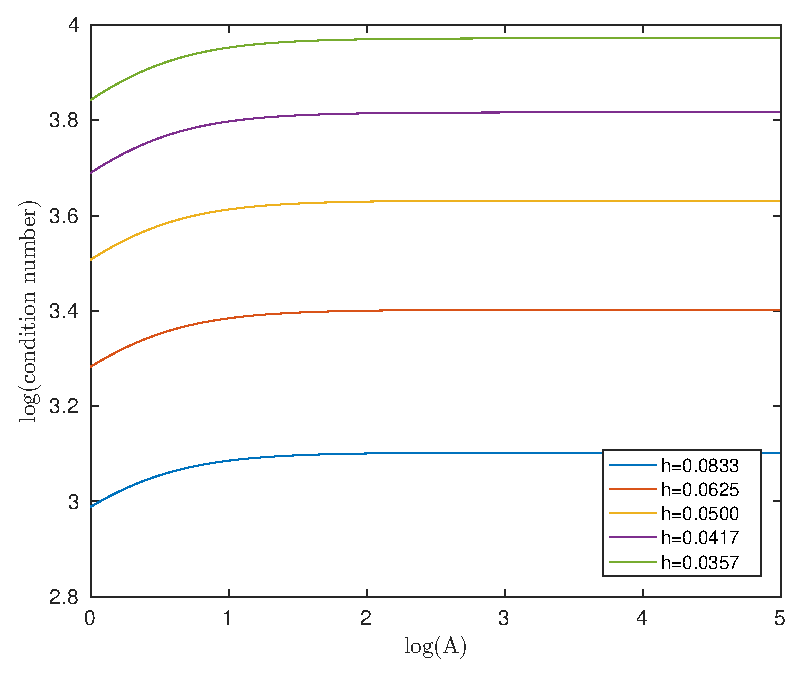
\includegraphics[width=\textwidth]{cond-A-2D-plinear-interface}
\caption{Constraint on interface}
\end{subfigure}
\caption{Scaled condition number, pseudo-linear interface}
\end{figure} 

Easy to spot that the scaled condition number behaves the same as a completely linear interface, and thus a complete analog with the one-dimensional case.

\subsection{Square interface}
Consider a square interface on $\Omega$. Here the interface $\beta$ is defined as \\
\[
\beta=
\begin{cases}
x=\frac{1}{4} & \frac{1}{4} \leq y \leq \frac{3}{4} \\
x=\frac{3}{4} & \frac{1}{4} \leq y \leq \frac{3}{4} \\
y=\frac{1}{4} & \frac{1}{4} \leq x \leq \frac{3}{4} \\
y=\frac{3}{4} & \frac{1}{4} \leq x \leq \frac{3}{4}
\end{cases}
\]

As illustrated by the following figure, consider a uniform mesh on $\Omega$. We take $a(x,y)=A$ when $(x,y)$ is inside the interface (excluding); and $a(x,y)=1$ otherwise. \\
\setlength{\unitlength}{1cm}
\thicklines
\begin{picture}(0,7)(-6.5,-0.5)
\put(0,0){\vector(1,0){6}}
\put(0,0){\vector(0,1){6}}
\multiput(0,0)(0,1){6}{\line(1,0){5}}
\multiput(0,0)(1,0){6}{\line(0,1){5}}
\put(0,5){\line(1,-1){5}}
\put(0,4){\line(1,-1){4}}
\put(0,3){\line(1,-1){3}}
\put(0,2){\line(1,-1){2}}
\put(0,1){\line(1,-1){1}}
\put(1,5){\line(1,-1){4}}
\put(2,5){\line(1,-1){3}}
\put(3,5){\line(1,-1){2}}
\put(4,5){\line(1,-1){1}}
\linethickness{1mm}
\put(1,1){\line(1,0){3}}
\put(1,1){\line(0,1){3}}
\put(1,4){\line(1,0){3}}
\put(4,4){\line(0,-1){3}}
\put(6,-0.3){$x$}
\put(-0.3,6){$y$}
\end{picture}

Consider the scaled condition number of the global stiffness matrix. Similar to the linear interface problem, we first put Neumann boundary on all the boundary nodal points, then we impose some constraints.

\begin{figure}[h!]
\centering
\begin{subfigure}{0.4\textwidth}
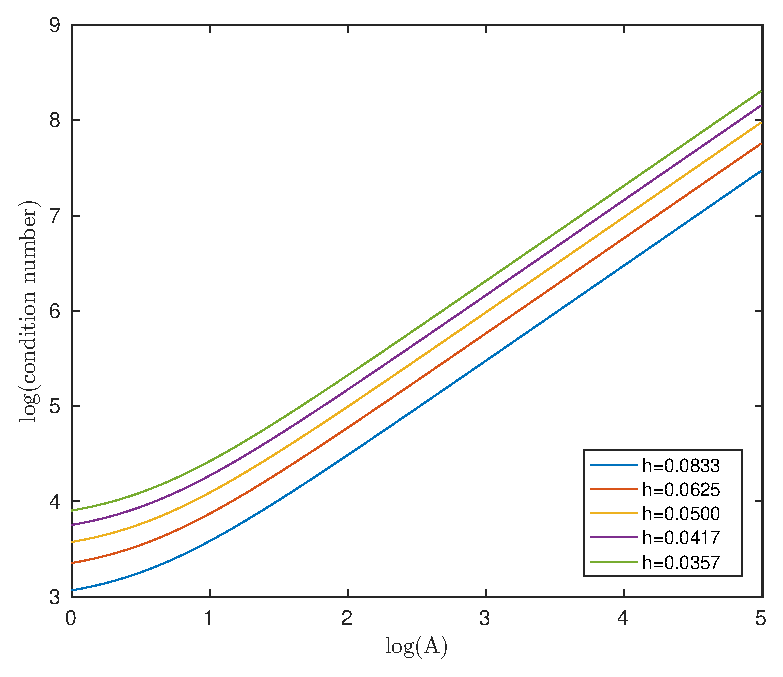
\includegraphics[width=\textwidth]{cond-A-2D-circular-DD}
\caption{Dirichlet-Dirichlet boundary}
\end{subfigure}
\hfill
\begin{subfigure}{0.4\textwidth}
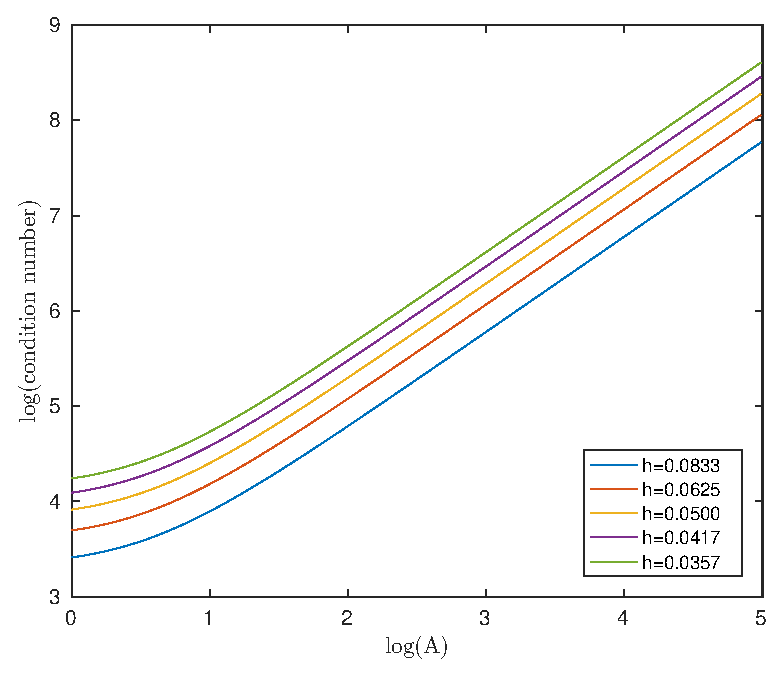
\includegraphics[width=\textwidth]{cond-A-2D-circular-DN}
\caption{Dirichlet-Neumann boundary}
\end{subfigure}
\vfill
\begin{subfigure}{0.4\textwidth}
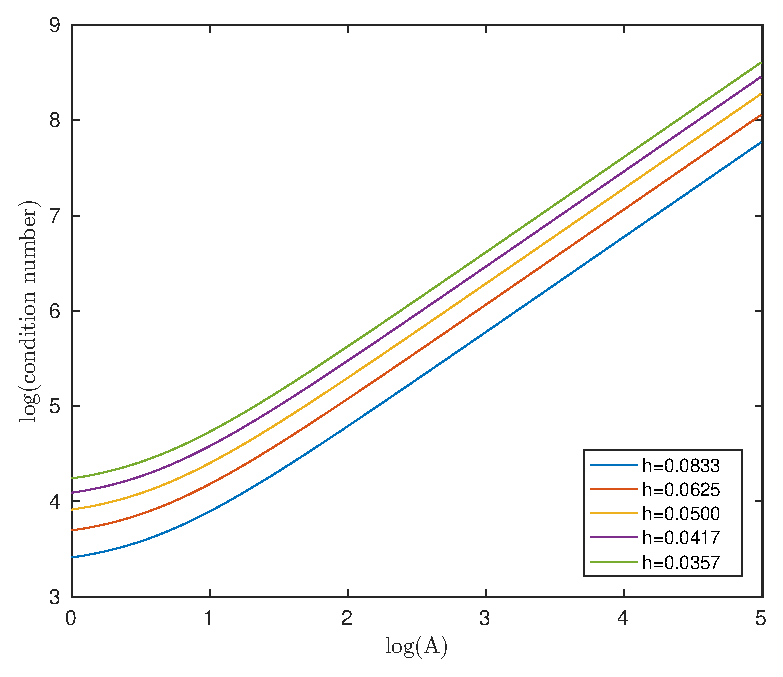
\includegraphics[width=\textwidth]{cond-A-2D-circular-ND}
\caption{Neumann-Dirichlet boundary}
\end{subfigure}
\caption{Scaled condition number, square interface $\beta$}
\end{figure}

Obviously if we only put constraints on the endpoints, i.e. on points $(0,0)$ or $(1,1)$, then the scaled condition number will be unbounded. Again, by saying Dirichlet-Dirichlet boundary, we mean putting constraints on  points $(0,0)$ and $(1,1)$. Likewise, we put a constraint on point $(0,0)$ to simulate Dirichlet-Neumann boundary, and we put a constraint on point $(1,1)$ to simulate Neumann-Dirichlet boundary.

However, like in the linear interface two-dimensional problem, if we put a constraint only on the interface, the scaled condition number is bounded.
\begin{figure}[h!]
\centering
\includegraphics[scale=0.55]{cond-A-2D-circular-interface}
\caption{Scaled condition number, square interface $\beta$, constraint on $(\frac{1}{4}, \frac{1}{4})$}
\end{figure}

Similarly, consider a pseudo-square interface that has a distortion on $\beta$. \\
\setlength{\unitlength}{1cm}
\thicklines
\begin{picture}(0,7.5)(-6,0)
\multiput(0,0)(0,1){7}{\line(1,0){6}}
\multiput(0,0)(1,0){7}{\line(0,1){6}}
\put(0,0){\vector(1,0){7}}
\put(0,0){\vector(0,1){7}}
\put(0,6){\line(1,-1){6}}
\put(0,5){\line(1,-1){5}}
\put(0,4){\line(1,-1){4}}
\put(0,3){\line(1,-1){3}}
\put(0,2){\line(1,-1){2}}
\put(0,1){\line(1,-1){1}}
\put(1,6){\line(1,-1){5}}
\put(2,6){\line(1,-1){4}}
\put(3,6){\line(1,-1){3}}
\put(4,6){\line(1,-1){2}}
\put(5,6){\line(1,-1){1}}
\linethickness{1mm}
\put(2,1){\line(1,0){3}}
\put(2,1){\line(0,1){1}}
\put(2,2){\line(-1,0){1}}
\put(1,2){\line(0,1){1}}
\put(1,3){\line(1,0){1}}
\put(2,3){\line(0,1){2}}
\put(2,5){\line(1,0){3}}
\put(5,5){\line(0,-1){4}}
\put(7,-0.3){$x$}
\put(-0.3,7){$y$}
\end{picture}

Like in the completely circular case, we obtain
\begin{figure}[h!]
\centering
\begin{subfigure}{0.4\textwidth}
\includegraphics[width=\textwidth]{cond-A-2D-pcircular-DD}
\caption{Dirichlet-Dirichlet boundary}
\end{subfigure}
\hfill
\begin{subfigure}{0.4\textwidth}
\includegraphics[width=\textwidth]{cond-A-2D-pcircular-DN}
\caption{Dirichlet-Neumann boundary}
\end{subfigure}
\vfill
\begin{subfigure}{0.4\textwidth}
\includegraphics[width=\textwidth]{cond-A-2D-pcircular-ND}
\caption{Neumann-Dirichlet boundary}
\end{subfigure}
\hfill
\begin{subfigure}{0.4\textwidth}
\includegraphics[width=\textwidth]{cond-A-2D-pcircular-interface}
\caption{Constraint on $(\frac{1}{4},\frac{1}{4})$}
\end{subfigure}
\caption{Scaled condition number, pseudo-square interface}
\end{figure}

\section{Conclusion}
From the discussion above, we can see that for the contrast problem, the behavior of the FEM solution depends significantly on the boundary conditions we impose, i.e. Dirichlet boundary or Neumann boundary.

Specifically, for an equation with large contrast, imposing Neumann boundary can cause the scaled condition number of the global stiffness matrix to be unbounded, and consequently cause the FEM solution to be inaccurate. On the other hand, imposing Dirichlet boundary or simply put a constraint on the interface will result in a bounded condition number.

\section*{Acknowledgment}
The author would like to thank Dr.Ivo Babuska for his patience and great help throughout this  project.

\section*{References}
Babuska, Ivo. \textit{Finite Elements, An Introduction to the Method and Error Estimation}

\end{document}